% Edit only the text between matching begin and end lines.
\documentclass[11pt,a4paper]{article}
% Shared preamble for TMUA worked solutions. Local edits here are overwritten.

% Reproducible PDFs: no timestamps, no trailer id, no build-path details.
\ifdefined\pdfsuppressptexinfo
  \pdfsuppressptexinfo=-1
  \pdfinfoomitdate=1
  \pdftrailerid{}
\fi

\usepackage{graphicx}
\usepackage{mathtools}
\usepackage{amssymb}
\usepackage{amsmath}
\usepackage{amsthm}
\usepackage{enumitem}
\usepackage{microtype}
\usepackage[table]{xcolor}
\usepackage{array}
\usepackage{booktabs}
\usepackage{tabularx}
\usepackage{longtable}
\usepackage{ragged2e}
\usepackage{fancyhdr}
\usepackage{etoolbox}
\usepackage[
  a4paper,
  left=0.8in,
  right=1in,
  top=1in,
  bottom=0.5in,
  headheight=14pt,
  headsep=0.4in
]{geometry}

\usepackage{pgfplots}
\pgfplotsset{compat=1.18}
\usepgfplotslibrary{fillbetween, polar}
\usetikzlibrary{calc, positioning}
\usetikzlibrary{angles, quotes}
\usetikzlibrary{arrows.meta}
\usetikzlibrary{decorations.pathreplacing, decorations.markings}
\usetikzlibrary{patterns}
\usetikzlibrary{intersections}

\usepackage{tocloft}
\usepackage[hidelinks]{hyperref}
\hypersetup{pdfauthor={danieljsmith.org}, pdfcreator={}, pdfsubject={}, pdfkeywords={}}
\urlstyle{same}
\tocloftpagestyle{djssolutions}
\setlength{\cftbeforesubsecskip}{2pt}
\setlength{\cftsubsecindent}{1.5em}
\setlength{\cftsubsecnumwidth}{0pt}
\renewcommand{\cftsubsecfont}{\small\color{black}}
\renewcommand{\cftsubsecpagefont}{\small\color{black}}
\renewcommand{\cftsubsecleader}{\hfill}

% `most` carries the breakable and enhanced libraries the solution box needs.
\usepackage[most]{tcolorbox}
\definecolor{scarlet}{RGB}{205, 40, 75}

\setlength{\parindent}{0pt}

% \djsSolutionsSetup{<paper title>}, called once after this file.
\newcommand{\djsSolnPaperTitle}{}
\newcommand{\djsSolutionsSetup}[1]{%
  \hypersetup{pdftitle={#1 Solutions}}%
  \renewcommand{\djsSolnPaperTitle}{#1}}

% The header appears only on the contents page and each question's opening
% page. Continuation pages use the empty default style.
\fancypagestyle{djssolutions}{%
  \fancyhead{}%
  \fancyfoot{}%
  \renewcommand{\headrulewidth}{0.9pt}%
  \fancyhead[L]{\textit{Solutions} - \djsSolnPaperTitle}%
  \fancyhead[R]{\href{https://danieljsmith.org}{danieljsmith.org}}%
}
\pagestyle{empty}

\newcolumntype{Y}{>{\RaggedRight\arraybackslash}X}

% Question layout, identical to the question paper's.
\newcommand{\djsTocTopic}[1]{%
  \ifblank{#1}{}{%
    \texorpdfstring
      {\hspace{0.9em}{\footnotesize\itshape\color{black!45}#1}}
      { \textendash\ #1}}}
\newcommand{\djsTopicLine}[1]{%
  \ifblank{#1}{}{%
    {\raggedleft\footnotesize\itshape\color{black!45}#1\par}%
    \vspace{-0.6\baselineskip}}}
\newcommand{\questionitem}[1][]{%
  \item\phantomsection
  \addcontentsline{toc}{subsection}{%
    Question \number\value{enumi}\protect\djsTocTopic{#1}}%
}
\renewcommand{\contentsname}{Questions}
\newcommand{\djsFrontMatter}{%
  \vspace*{20pt}%
  \tableofcontents
  \newpage
}

% The solution body: a white breakable box with a left scarlet rule. The
% rule continues onto a continuation page and stops where the solution
% stops, then turns into a short horizontal of the same weight so the
% solution visibly ends. The argument is the answer label.
\newcommand{\djsSolutionAnswer}[1]{%
  {\color{scarlet}\bfseries Answer\ \ #1}}
\newtcolorbox{djsSolution}[1]{%
  enhanced, breakable, frame hidden, sharp corners, colback=white,
  height fixed for=first and middle, height fill,
  extras unbroken and last={natural height},
  borderline west={2.2pt}{0pt}{scarlet},
  left=11pt, right=0pt, top=5pt, bottom=13pt,
  before skip=13pt, after skip=4pt,
  overlay unbroken and last={%
    \fill[scarlet] (frame.south west)
      rectangle ([xshift=3.5cm, yshift=2.2pt]frame.south west);},
  before upper={\setlength{\parskip}{6pt}%
                {\color{scarlet}\bfseries Solution}%
                \hfill\djsSolutionAnswer{#1}\par\vspace{4pt}}}

% Solution figures sit inside the box and are drawn smaller than question
% figures; \scalebox shrinks node text with the drawing.
\newcommand{\SolnFigureScale}{0.85}
\newsavebox{\djsSolnFigureBox}
\newenvironment{djsSolutionFigure}
  {\par\vspace{4pt}\begin{center}\begin{lrbox}{\djsSolnFigureBox}}
  {\end{lrbox}\scalebox{\SolnFigureScale}{\usebox{\djsSolnFigureBox}}%
   \end{center}\vspace{2pt}\par}

\djsSolutionsSetup{TMUA Set A Paper 2}
\begin{document}
\thispagestyle{djssolutions}
\djsFrontMatter
\clearpage
\thispagestyle{djssolutions}
\vspace*{8pt}
\djsTopicLine{Proof \& Error Analysis}
\begin{enumerate}[label=\textbf{\arabic*.},leftmargin=*,itemsep=0pt,start=1]
\questionitem[Proof \& Error Analysis]
% begin q000646 stem

Let $x$ and $y$ be real numbers.

A student attempts to prove the following claim: \begin{center}
\begin{minipage}{0.82\linewidth}
\centering
\textbf{Claim:} If $x+y\geq2$ then $x^2+y^2\ge 2$
\end{minipage}
\end{center} The student's attempt is as follows:

\[
\begin{array}{@{}rl@{}}
\textbf{Line 1:} &
\text{Since }x+y\ge2,\text{ at least one of }x\text{ and }y\text{ is at least }1. \\[-1pt]
&
\text{Assume }x\ge1;\text{ the other case is the same with }x\text{ and }y\text{ swapped.} \\[5pt]

\textbf{Line 2:} &
\text{From }x+y\ge2\text{ we get }y\ge2-x \\[5pt]

\textbf{Line 3:} &
\text{Therefore }y^2\ge(2-x)^2 \\[5pt]

\textbf{Line 4:} &
\text{Hence }x^2+y^2\ge x^2+(2-x)^2 \\[5pt]

\textbf{Line 5:} &
\text{Now }x^2+(2-x)^2=2(x-1)^2+2,\text{ and this is at least }2. \\[5pt]

\textbf{Line 6:} &
\text{Therefore }x^2+y^2\ge2,\text{ as claimed.}\\[5pt]
\end{array}
\]


Which of the following best describes the argument?
% end q000646 stem

\par\vspace*{12pt}
\begin{tabularx}{\linewidth}{@{}>{\bfseries}l Y@{}}
A &
% begin q000646 choice A
Line 1 contains the first error.
% end q000646 choice A
\\[0.8em]
B &
% begin q000646 choice B
Line 2 contains the first error.
% end q000646 choice B
\\[0.8em]
C &
% begin q000646 choice C
Line 3 contains the first error.
% end q000646 choice C
\\[0.8em]
D &
% begin q000646 choice D
Line 4 contains the first error.
% end q000646 choice D
\\[0.8em]
E &
% begin q000646 choice E
Line 5 contains the first error.
% end q000646 choice E
\\[0.8em]
F &
% begin q000646 choice F
The argument is a correct proof of the claim.
% end q000646 choice F
\\[0.8em]
G &
% begin q000646 choice G
The argument contains no error, but the claim is false.
% end q000646 choice G
\\
\end{tabularx}

\begin{djsSolution}{C}
% begin q000646 solution
The claim looks plausible. No counterexample is readily apparent. Instead, lets check each line in order.

Line 1 is valid: if both $x<1$ and $y<1$, then $x+y<2$. Swapping $x$ and $y$ does not change the claim, so it is enough to consider $x\geq1$. 

Line 2 is also valid: subtracting $x$ from $x+y\geq2$ gives $y\geq2-x$.

Line 3 is the first error. Squaring does not always preserve an inequality when negative numbers are involved. 

For example, take $x=3$ and $y=-\dfrac12$. Then $2-x=-1$, $(2-x)^2=1$ and $y^2=\dfrac{1}{4}$.

Now we see that squaring does \textbf{not} maintain the direction of the inequality:
\[
-\dfrac12\geq-1\]
but
\[
\left(-\dfrac{1}{2}\right)^2=\dfrac14<(-1)^2=1
\]

So squaring reversed the inequality. This is a counterexample to the step on line 3, not to the claim itself.

Therefore the first error is on line 3, so the correct option is \textbf{C}. \\

\textit{Remark:} (optional)

To see why the claim is true despite the faulty proof, note the algebraic fact:
\begin{align*}
(x+y)^2+(x-y)^2 &= (x^2 + 2xy + y^2) + (x^2-2xy+y^2)\\
                &= 2x^2 + 2y^2 \\
                &= 2(x^2+y^2)
\end{align*}
so \((x+y)^2+(x-y)^2 = 2(x^2+y^2)\)

Since \((x-y)^2\geq0\) it follows that 
\[
2(x^2+y^2) =(x+y)^2+(x-y)^2 \geq (x+y)^2
\]

So \(2(x^2+y^2)\geq(x+y)^2\) or equivalently \(x^2+y^2\geq\dfrac{(x+y)^2}{2}\)

Finally, we are told that \(x+y\geq2\) so \((x+y)^2\geq2^2=4\) (we are allowed to square an inequality when both sides are positive)

Therefore
\[x^2+y^2\geq \dfrac{2^2}{2}=2\]

Thus, it is true that if $x+y\geq2$ then $x^2+y^2\geq2$, but the given argument is not a correct proof of that fact. 

Providing a correct proof was, of course, not a requirement of the question. But it explains why counterexamples were hard to find. False proofs of correct statements are some of the hardest error analysis questions.
% end q000646 solution
\end{djsSolution}
\end{enumerate}
\clearpage
\thispagestyle{djssolutions}
\vspace*{8pt}
\djsTopicLine{Trigonometry}
\begin{enumerate}[label=\textbf{\arabic*.},leftmargin=*,itemsep=0pt,start=2]
\questionitem[Trigonometry]
% begin q000636 stem
In quadrilateral $ABCD$, the diagonal $AC$ divides the figure into two right-angled triangles, $\triangle ABC$ and $\triangle ACD$.

\begin{itemize}
    \item In $\triangle ABC$, $\angle ABC = 90^\circ$, $\angle BAC = 30^\circ$, and $AB = \sqrt{6}\text{ cm}$
    \item In $\triangle ACD$, $\angle ACD = 90^\circ$, and $\tan(\angle CAD) = \dfrac{1}{\sqrt{2}}$
\end{itemize}

What is the area of quadrilateral $ABCD$, in $\text{cm}^2$? \\
% end q000636 stem

\par\vspace*{12pt}
\begin{tabularx}{\linewidth}{@{}>{\bfseries}l Y@{}}
A &
% begin q000636 choice A
$\sqrt{3} + \sqrt{2}$
% end q000636 choice A
\\[0.8em]
B &
% begin q000636 choice B
$\sqrt{3} + 2\sqrt{2}$
% end q000636 choice B
\\[0.8em]
C &
% begin q000636 choice C
$2\sqrt{3} + \sqrt{2}$
% end q000636 choice C
\\[0.8em]
D &
% begin q000636 choice D
$2\sqrt{3} + 2\sqrt{2}$
% end q000636 choice D
\\[0.8em]
E &
% begin q000636 choice E
$\sqrt{3} + 4\sqrt{2}$
% end q000636 choice E
\\[0.8em]
F &
% begin q000636 choice F
$2\sqrt{3} + 4\sqrt{2}$
% end q000636 choice F
\\
\end{tabularx}

\begin{djsSolution}{B}
% begin q000636 solution
Let $\theta=\angle CAD$, so $\tan\theta=\dfrac{1}{\sqrt{2}}$

The situation can be explained by the diagram:

\begin{djsSolutionFigure}
% begin q000636 figure F1
\begin{tikzpicture}[scale=2.5]
\coordinate (A) at (0,0);
\coordinate (C) at ({2*sqrt(2)},0);
\coordinate (B) at ({3*sqrt(2)/2},{-sqrt(6)/2});
\coordinate (D) at ($(C)+(0,2)$);

\draw[thick,black] (A)--(B)--(C)--(D)--cycle;
\draw[thick,black] (A)--(C);
\pic[draw,angle radius=4mm] {right angle=A--B--C};
\pic[draw,angle radius=4mm] {right angle=A--C--D};
\pic["$30^\circ$",draw,angle radius=8mm,angle eccentricity=1.5] {angle=B--A--C};
\pic["$\theta$",draw,angle radius=8mm,angle eccentricity=1.45] {angle=C--A--D};

\node[below left=2pt] at (A) {$A$};
\node[below=3pt] at (B) {$B$};
\node[below right=2pt] at (C) {$C$};
\node[above=2pt] at (D) {$D$};
\path (A)--(B) node[midway,below left=2pt] {$\sqrt{6}\,\mathrm{cm}$};
\end{tikzpicture}
% end q000636 figure F1
\end{djsSolutionFigure}

In right-angled triangle $ABC$, the side opposite the $30^\circ$ angle is $BC$ and the adjacent side is $AB$. Hence
\[
\tan 30^\circ=\frac{BC}{AB}=\frac{BC}{\sqrt{6}}=\frac{1}{\sqrt{3}}
\]
Therefore
\[
BC=\frac{\sqrt{6}}{\sqrt{3}}=\sqrt{2}\text{ cm}
\]
Pythagoras now gives the shared diagonal:
\[
AC^2=AB^2+BC^2=6+2=8 \quad\implies
\quad AC=2\sqrt{2}\text{ cm}
\]

In right-angled triangle $ACD$, $CD$ is opposite $\theta$ and $AC$ is adjacent to it. Thus
\[
\tan\theta=\frac{CD}{AC}=\frac{CD}{2\sqrt{2}}=\frac{1}{\sqrt{2}}
\quad\implies\quad CD=2\text{ cm}
\]

\begin{djsSolutionFigure}
% begin q000636 figure F2
\begin{tikzpicture}[scale=2.5]
\coordinate (A) at (0,0);
\coordinate (C) at ({2*sqrt(2)},0);
\coordinate (B) at ({3*sqrt(2)/2},{-sqrt(6)/2});
\coordinate (D) at ($(C)+(0,2)$);

\draw[thick,black] (A)--(B)--(C)--(D)--cycle;
\draw[thick,black] (A)--(C);
\pic[draw,angle radius=4mm] {right angle=A--B--C};
\pic[draw,angle radius=4mm] {right angle=A--C--D};
\pic["$30^\circ$",draw,angle radius=8mm,angle eccentricity=1.5] {angle=B--A--C};
\pic["$\theta$",draw,angle radius=8mm,angle eccentricity=1.45] {angle=C--A--D};

\node[below left=2pt] at (A) {$A$};
\node[below=3pt] at (B) {$B$};
\node[below right=2pt] at (C) {$C$};
\node[above=2pt] at (D) {$D$};
\path (A)--(B) node[midway,below left=2pt] {$\sqrt{6}\,\mathrm{cm}$};
\path (B)--(C) node[midway,below right=2pt,text=red] {$\sqrt{2}\,\mathrm{cm}$};
\path (A)--(C) node[midway,above=4pt,text=red] {$2\sqrt{2}\,\mathrm{cm}$};
\path (C)--(D) node[midway,right=4pt,text=red] {$2\,\mathrm{cm}$};
\end{tikzpicture}
% end q000636 figure F2
\end{djsSolutionFigure}

The two right-angled triangles have perpendicular side pairs $AB,BC$ and $AC,CD$. Their areas are
\[
\begin{aligned}
\text{Area of }ABC&=\frac12 AB\times BC
=\frac12\sqrt{6}\times\sqrt{2}=\sqrt{3}\text{ cm}^2,\\
\text{Area of }ACD&=\frac12 AC\times CD
=\frac12(2\sqrt{2})\times2=2\sqrt{2}\text{ cm}^2.
\end{aligned}
\]
Adding them gives $\sqrt{3}+2\sqrt{2}\text{ cm}^2$, so the correct option is \textbf{B}.
% end q000636 solution
\end{djsSolution}
\end{enumerate}
\clearpage
\thispagestyle{djssolutions}
\vspace*{8pt}
\djsTopicLine{Proof \& Error Analysis}
\begin{enumerate}[label=\textbf{\arabic*.},leftmargin=*,itemsep=0pt,start=3]
\questionitem[Proof \& Error Analysis]
% begin q000681 stem
Consider the following claim and attempted proof.

\begin{center}
\begin{minipage}{0.82\linewidth}
\centering
\textbf{Claim:} Let $f(x)$ be a quadratic polynomial. If $\displaystyle\int_{-1}^{1} f(x)\,\mathrm{d}x = 0$, then the graph of $y = f(x)$ must intersect the $x$-axis at two distinct points in the interval $-1 < x < 1$.
\end{minipage}
\end{center}
Attempted proof:
\[
\begin{array}{@{}rl@{}}
\textbf{Line 1} & \text{Let } f(x) = ax^2 + bx + c\text{, where } a, b, c \text{ are real constants with } a \ne 0 \\[5pt]
\textbf{Line 2} & \text{Evaluating the integral gives } \displaystyle\int_{-1}^{1} f(x)\,\mathrm{d}x = \frac{2a}{3} + 2c = 0\text{, so } c = -\frac{a}{3} \\[12pt]
\textbf{Line 3} & \text{The discriminant is } b^2-4ac=b^2+\frac{4a^2}{3}>0\text{, so }f(x)=0\text{ has two distinct real roots} \\[7pt]
\textbf{Line 4} & \text{Writing these roots as }x_1\text{ and }x_2\text{, we have }x_1x_2=\frac{c}{a}=-\frac{1}{3} \\[7pt]
\textbf{Line 5} & \text{Since } |x_1 x_2| = \frac{1}{3} < 1\text{, it follows that } |x_1| < 1 \text{ and } |x_2| < 1 \\[7pt]
\textbf{Line 6} & \text{Therefore, both roots lie in the interval } -1 < x < 1\\[5pt]
\end{array}
\]

Which line of the proof contains the first error?
% end q000681 stem

\par\vspace*{12pt}
\begin{tabularx}{\linewidth}{@{}>{\bfseries}l Y@{}}
A &
% begin q000681 choice A
Line 1
% end q000681 choice A
\\[0.8em]
B &
% begin q000681 choice B
Line 2
% end q000681 choice B
\\[0.8em]
C &
% begin q000681 choice C
Line 3
% end q000681 choice C
\\[0.8em]
D &
% begin q000681 choice D
Line 4
% end q000681 choice D
\\[0.8em]
E &
% begin q000681 choice E
Line 5
% end q000681 choice E
\\[0.8em]
F &
% begin q000681 choice F
Line 6
% end q000681 choice F
\\[0.8em]
G &
% begin q000681 choice G
There is no error, the proof is correct as written.
% end q000681 choice G
\\
\end{tabularx}

\begin{djsSolution}{E}
% begin q000681 solution
An integral can be zero when the area above the $x$-axis balances the area below it. 

The sketch shows how this might happen for a quadratic with only one root between $-1$ and $1$, indicating that the claim is false:

\begin{djsSolutionFigure}
% begin q000681 figure F1
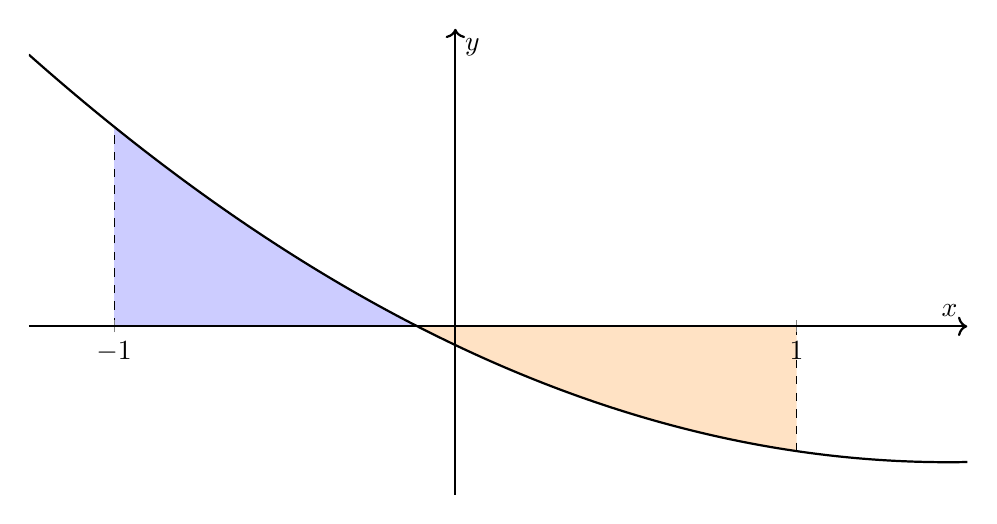
\begin{tikzpicture}
\pgfmathsetmacro{\innerroot}{-1/9}
\pgfmathsetmacro{\yminus}{(-1-3)*(-1+1/9)}
\pgfmathsetmacro{\yplus}{(1-3)*(1+1/9)}
\begin{axis}[
    width=13.5cm, height=7.5cm,
    xmin=-1.25, xmax=1.5,
    ymin=-3, ymax=5.3,
    axis lines=middle,
    axis line style={->, thick, black},
    axis on top,
    xlabel={$x$}, ylabel={$y$},
    xtick={-1,0,1},
    xticklabels={$-1$,$0$,$1$},
    ytick=\empty,
    clip=true,
]
\addplot[draw=none, name path=leftcurve, domain=-1:\innerroot, samples=50] {(x-3)*(x+1/9)};
\addplot[draw=none, name path=leftbase, domain=-1:\innerroot] {0};
\addplot[fill=blue!20, draw=none] fill between[of=leftcurve and leftbase];
\addplot[draw=none, name path=rightcurve, domain=\innerroot:1, samples=70] {(x-3)*(x+1/9)};
\addplot[draw=none, name path=rightbase, domain=\innerroot:1] {0};
\addplot[fill=orange!23, draw=none] fill between[of=rightcurve and rightbase];
\draw[thin, dashed] (axis cs:-1,0) -- (axis cs:-1,\yminus);
\draw[thin, dashed] (axis cs:1,0) -- (axis cs:1,\yplus);
\addplot[thick, black, domain=-1.25:3.3, samples=200] {(x-3)*(x+1/9)};
\end{axis}
\end{tikzpicture}
% end q000681 figure F1
\end{djsSolutionFigure}

We could search for a specific quadratic with this property and plug it in line-by-line to find the error, but finding the quadratic itself sounds like a lot of effort.

Therefore, we will analyse the proof line-by-line.

Line 1 gives the general form of a quadratic. $a\ne0$ is required so the $x^2$ term doesn't cancel. Line 1 is correct.

In Line 2, the $bx$ term contributes zero because its integral from $-1$ to $1$ cancels on either side of $0$. Thus
\[\int_{-1}^{1}(ax^2+bx+c)\,\mathrm{d}x=\left[\frac{ax^3}{3}+\frac{bx^2}{2}+cx\right]_{-1}^{1}=\frac{2a}{3}+2c=0\]
so $c=-a/3$, as stated. Line 2 is correct.

Using this value of $c$, Line 3 gives
\[b^2-4ac=b^2+\frac{4a^2}{3}>0\]
because $a\ne0$. There are therefore two distinct real roots because the discriminant is strictly positive. Line 3 is correct.

Line 4 correctly uses the product of the roots formula, $x_1x_2=\dfrac{c}{a}$ to obtain
\[x_1x_2=-\frac13\]
The mistake is in Line 5: a product with absolute value less than $1$ does not require both factors to have absolute value less than $1$. \\

For example, $x_1=3$ and $x_2=\dfrac19$ give $|x_1x_2|=\dfrac13$, although $|x_1| = 3>1$

Even retaining the negative product from Line 4, $x_1=3$ and $x_2=-\dfrac19$ give $x_1x_2=-\dfrac13$, with one root outside the interval $-1\leq x\leq1$

The first error is therefore in Line 5, so the correct option is \textbf{E}.
% end q000681 solution
\end{djsSolution}
\end{enumerate}
\clearpage
\thispagestyle{djssolutions}
\vspace*{8pt}
\djsTopicLine{Exponentials \& Logarithms}
\begin{enumerate}[label=\textbf{\arabic*.},leftmargin=*,itemsep=0pt,start=4]
\questionitem[Exponentials \& Logarithms]
% begin q000046 stem
Let $a$ be a positive real number with $a \ne 1$

The equation \[ \log_a(3x-1) = 2 + \log_a(x+1) \] has exactly one real solution $x$

What is the complete range of all the possible values of $a$?
% end q000046 stem

\par\vspace*{12pt}
\begin{tabularx}{\linewidth}{@{}>{\bfseries}l Y@{}}
A &
% begin q000046 choice A
$0<a<\sqrt{3}$ and $a\ne 1$
% end q000046 choice A
\\[0.8em]
B &
% begin q000046 choice B
$a > 1$
% end q000046 choice B
\\[0.8em]
C &
% begin q000046 choice C
$a>0$ and $a \ne 1$
% end q000046 choice C
\\[0.8em]
D &
% begin q000046 choice D
No such $a$ exists
% end q000046 choice D
\\[0.8em]
E &
% begin q000046 choice E
$a=3$
% end q000046 choice E
\\[0.8em]
F &
% begin q000046 choice F
$a=\frac{1}{3}$
% end q000046 choice F
\\[0.8em]
G &
% begin q000046 choice G
$a>0$, $a \ne 1$ and $a \ne \sqrt{3}$
% end q000046 choice G
\\
\end{tabularx}

\begin{djsSolution}{A}
% begin q000046 solution
Subtracting $\log_a(x+1)$ from both sides gives
\[
\log_a(3x-1)-\log_a(x+1)=2
\]

Combining the logarithms,
\[
\log_a\left(\frac{3x-1}{x+1}\right)=2
\]

Hence, provided the original logarithms are defined,
\[
\frac{3x-1}{x+1}=a^2
\]

Multiplying through and rearranging,
\[
3x-1=a^2x+a^2
\]
\[
(3-a^2)x=1+a^2
\]

Hence, provided $3-a^2\ne0$, there is only one candidate solution
\[
x=\frac{1+a^2}{3-a^2}
\]

Note first that the denominator can never be zero, so $a=\sqrt{3}$ must be excluded from the answer.

Excluding $a=\sqrt3$ does not yet give option \textbf{G}: our candidate solution must also make both original logarithms defined (that is, we must make sure the insides of both logarithms are positive).

In particular, we must check this before deciding whether the range is \textbf{A} or a smaller set such as \textbf{F}.

Substituting the candidate solution into each logarithm's argument gives

\[x+1=\frac{4}{3-a^2}\qquad\text{and}\qquad 3x-1=\frac{4a^2}{3-a^2}\]

Both must be positive to ensure the original logarithms are defined. 

Because $a>0$, both numerators are positive, so each condition requires $3-a^2>0$. This gives $a<\sqrt3$. 

Conversely, every $a$ with $0<a<\sqrt3$ and $a\ne1$ makes both arguments positive and gives the unique solution found above. 

Hence the complete range is
\[0<a<\sqrt3,\qquad a\ne1\]
The correct option is \textbf{A}.
% end q000046 solution
\end{djsSolution}
\end{enumerate}
\clearpage
\thispagestyle{djssolutions}
\vspace*{8pt}
\djsTopicLine{Number}
\begin{enumerate}[label=\textbf{\arabic*.},leftmargin=*,itemsep=0pt,start=5]
\questionitem[Number]
% begin q000592 stem
A positive integer $n$ can be written as $n = 2^a3^b$ where $a$ and $b$ are non-negative integers. 

The number $n$ has exactly $12$ positive factors, counting $1$ and $n$ itself. 

Given that $n<200$, what is the greatest possible value of $n$?
% end q000592 stem

\par\vspace*{12pt}
\begin{tabularx}{\linewidth}{@{}>{\bfseries}l Y@{}}
A &
% begin q000592 choice A
$72$
% end q000592 choice A
\\[0.8em]
B &
% begin q000592 choice B
$96$
% end q000592 choice B
\\[0.8em]
C &
% begin q000592 choice C
$108$
% end q000592 choice C
\\[0.8em]
D &
% begin q000592 choice D
$144$
% end q000592 choice D
\\[0.8em]
E &
% begin q000592 choice E
$162$
% end q000592 choice E
\\[0.8em]
F &
% begin q000592 choice F
$486$
% end q000592 choice F
\\
\end{tabularx}

\begin{djsSolution}{C}
% begin q000592 solution
Since
\[
n=2^a3^b
\]
every positive factor of \(n\) is obtained by choosing a power of \(2\) from
\[
2^0,\,2^1,\ldots,\,2^a
\]
and independently choosing a power of \(3\) from
\[
3^0,\,3^1,\ldots,\,3^b
\]
Thus every positive factor has the form \(2^i3^j\), where there are \(a+1\) possible values of \(i\) and \(b+1\) possible values of \(j\). 

Therefore the total number of positive factors is \((a+1)(b+1)\) and the question then gives us that
\[
(a+1)(b+1)=12
\]

Test the choices from largest to smallest: the first one below $200$ that satisfies this equation must be the answer. 

Choice F is $486>200$, so it is too large. 

For the next three choices,
\[\begin{aligned}
162&=2^1 3^4 &&\text{gives }(1+1)(4+1)=10\neq12\\
144&=2^4 3^2 &&\text{gives }(4+1)(2+1)=15\neq12\\
108&=2^2 3^3 &&\text{gives }(2+1)(3+1)=12 \,\checkmark
\end{aligned}\]

Thus $108$ is the greatest eligible choice, so the answer is \textbf{C}.\\[5pt]

\textit{Alternative Solution:}

Let's try to obtain $108$ without testing the given options.

Since $2^8=256$ and $3^5=243$, the condition $n<200$ requires $a\leq7$ and $b\leq4$. 

The possible factor pairs for $(a+1)(b+1)=12$ are $1$ and $12$, $2$ and $6$, or $3$ and $4$, in either order. 

The bounds $a\leq7$ and $b\leq4$ rule out all but these cases:
\[\begin{array}{c|c|c}
a&b&2^a3^b\\ \hline
2&3&108\\
3&2&72\\
5&1&96
\end{array}\]
The largest is $108$, so the answer is again \textbf{C}. \\

Testing the solutions from the largest first is clearly more efficient here. Even if it a feels a little like cheating, it is an entirely valid and highly strategic move in a time-pressured multiple choice test.
% end q000592 solution
\end{djsSolution}
\end{enumerate}
\clearpage
\thispagestyle{djssolutions}
\vspace*{8pt}
\djsTopicLine{Proof \& Error Analysis}
\begin{enumerate}[label=\textbf{\arabic*.},leftmargin=*,itemsep=0pt,start=6]
\questionitem[Proof \& Error Analysis]
% begin q000648 stem
Let $a$ and $b$ be real numbers. A student attempts to prove the following claim: 
\begin{center} \begin{minipage}{0.82\linewidth} \centering \textbf{Claim:} If $a+b$ and $ab$ are both integers, then $a$ and $b$ are both integers. \end{minipage} \end{center}

The student's attempt is as follows:\[
\begin{array}{@{}rl@{}}
\textbf{I} &
\text{$a$ and $b$ are the two solutions of }
t^2-(a+b)t+ab=0 \\[10pt]

\textbf{II} &
\text{Write }s=a+b\text{ and }p=ab,\text{ so }s\text{ and }p\text{ are integers and} \\[-1pt]
&
\displaystyle
\text{the two solutions are }
t=\frac{s\pm\sqrt{s^2-4p}}{2} \\[10pt]

\textbf{III} &
\text{Since }a\text{ and }b\text{ are real, }s^2-4p\geq0 \\[10pt]

\textbf{IV} &
\text{Also }s^2-4p\text{ is an integer, so }\sqrt{s^2-4p}
\text{ is either an integer or an irrational number.} \\[10pt]

\textbf{V} &
\text{If }\sqrt{s^2-4p}\text{ were irrational, then }a\text{ would be irrational,} \\[-1pt]
&
\text{and so }a+b\text{ would be irrational, contradicting the fact that }
a+b\text{ is an integer.} \\[10pt]

\textbf{VI} &
\text{Hence }\sqrt{s^2-4p}\text{ is an integer, so }
s\pm\sqrt{s^2-4p}\text{ is an integer,} \\[-1pt]
&
\text{and therefore }a\text{ and }b\text{ are both integers.}
\end{array}
\]

Which of the following best describes this attempt?
% end q000648 stem

\par\vspace*{12pt}
\begin{tabularx}{\linewidth}{@{}>{\bfseries}l Y@{}}
A &
% begin q000648 choice A
It is completely correct.
% end q000648 choice A
\\[0.8em]
B &
% begin q000648 choice B
It is incorrect, and the first error is on line I.
% end q000648 choice B
\\[0.8em]
C &
% begin q000648 choice C
It is incorrect, and the first error is on line II.
% end q000648 choice C
\\[0.8em]
D &
% begin q000648 choice D
It is incorrect, and the first error is on line III.
% end q000648 choice D
\\[0.8em]
E &
% begin q000648 choice E
It is incorrect, and the first error is on line IV.
% end q000648 choice E
\\[0.8em]
F &
% begin q000648 choice F
It is incorrect, and the first error is on line V.
% end q000648 choice F
\\[0.8em]
G &
% begin q000648 choice G
It is incorrect, and the first error is on line VI.
% end q000648 choice G
\\
\end{tabularx}

\begin{djsSolution}{F}
% begin q000648 solution
A counterexample to the claim is $a=\sqrt2$ and $b=-\sqrt2$. 

Neither is an integer, but
\[
a+b=0,\qquad ab=-2
\]

Both required quantities are integers, so we can run this example through the student's argument to find the first faulty line.

Lines I works. With these choices the quadratic becomes $t^2-2$ which clearly has roots $\pm\sqrt2$:
\begin{align*}
t^2-(a+b)t+ab&=t^2-2\\&=(t-\sqrt2)(t+\sqrt2)
\end{align*}

Line II also works. The quadratic formula gives the same result for the roots:

\begin{align*}
t&=\frac{0\pm\sqrt{0^2-4(-2)}}{2}=\pm\sqrt2
\end{align*}

Lines III and IV also hold. The discriminant is

\[
s^2-4p=0^2-4(-2)=8\geq0
\]

The square root of the discriminant \(\sqrt{s^2-4p} = \sqrt8=2\sqrt2 \) is irrational, as line IV allows.

The first error is on line V:

Although $a=\sqrt2$ is irrational, it does not follow that $a+b$ is irrational: $b$ is irrational too, and the two terms cancel to give $a+b=0$, a rational number.

The student's argument first draws a false conclusion from true statements on line V, so the correct option is \textbf{F}.
% end q000648 solution
\end{djsSolution}
\end{enumerate}
\clearpage
\thispagestyle{djssolutions}
\vspace*{8pt}
\djsTopicLine{Geometry}
\begin{enumerate}[label=\textbf{\arabic*.},leftmargin=*,itemsep=0pt,start=7]
\questionitem[Geometry]
% begin q000569 stem
Triangle $ABC$ is right-angled at $A$, with $AB=6\,\mathrm{cm}$ and $AC=8\,\mathrm{cm}$.

Semicircles are drawn with $AB$, $AC$ and $BC$ as diameters, as shown. The semicircle on $BC$ is on the same side of the line $BC$ as $A$. The portions of the other two semicircles that lie outside the semicircle on $BC$ are shaded.

What is the total shaded area, in $\mathrm{cm}^2$?
% end q000569 stem

\begin{center}
% begin q000569 diagram
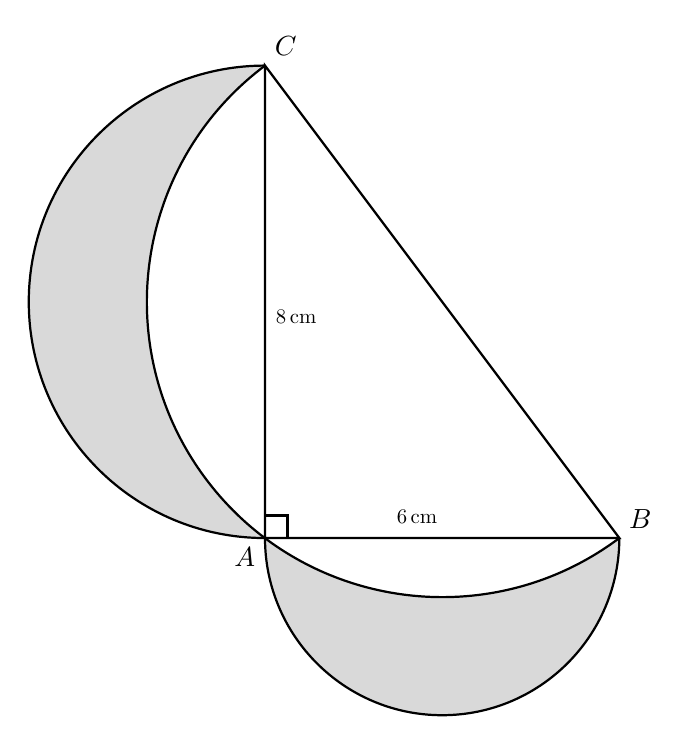
\begin{tikzpicture}[scale=0.75]
\def\AB{6}
\def\AC{8}
\def\ra{0.38}
\pgfmathsetmacro{\rAB}{\AB/2}
\pgfmathsetmacro{\rAC}{\AC/2}
\pgfmathsetmacro{\rBC}{sqrt(\AB*\AB+\AC*\AC)/2}
\pgfmathsetmacro{\alphaang}{atan(\AC/\AB)}
\pgfmathsetmacro{\angB}{-\alphaang}
\pgfmathsetmacro{\angA}{\alphaang-180}
\pgfmathsetmacro{\angC}{-\alphaang-180}

\coordinate (A) at (0,0);
\coordinate (B) at (\AB,0);
\coordinate (C) at (0,\AC);

% Shaded lune adjacent to AB
\path[fill=gray!30]
  (A) arc[start angle=180,end angle=360,radius=\rAB]
  arc[start angle=\angB,end angle=\angA,radius=\rBC]
  -- cycle;

% Shaded lune adjacent to AC
\path[fill=gray!30]
  (A) arc[start angle=-90,end angle=-270,radius=\rAC]
  arc[start angle=\angC,end angle=\angA,radius=\rBC]
  -- cycle;

% Three semicircular arcs
\draw[thick, black] (A) arc[start angle=180,end angle=360,radius=\rAB];
\draw[thick, black] (A) arc[start angle=-90,end angle=-270,radius=\rAC];
\draw[thick, black] (B) arc[start angle=\angB,end angle=\angC,radius=\rBC];

% Triangle and its diameters
\draw[thick, black] (A) -- (B) -- (C) -- cycle;

% Right-angle marker
\coordinate (RAx) at ($(A)+(\ra,0)$);
\coordinate (RAxy) at ($(A)+(\ra,\ra)$);
\coordinate (RAy) at ($(A)+(0,\ra)$);
\draw[thick] (RAx) -- (RAxy) -- (RAy);

% Labels
\node[below left] at (A) {$A$};
\node[above right] at (B) {$B$};
\node[above right] at (C) {$C$};
\node[midway, above, yshift=100pt, xshift=15pt] at ($(A)!0.5!(B)$) {$8\,\mathrm{cm}$};
\node[midway, right, yshift=10pt, xshift=60pt] at ($(A)!0.5!(C)$) {$6\,\mathrm{cm}$};
\end{tikzpicture}
% end q000569 diagram
\end{center}

\par\vspace*{12pt}
\begin{tabularx}{\linewidth}{@{}>{\bfseries}l Y@{}}
A &
% begin q000569 choice A
$12$
% end q000569 choice A
\\[0.8em]
B &
% begin q000569 choice B
$24$
% end q000569 choice B
\\[0.8em]
C &
% begin q000569 choice C
$30$
% end q000569 choice C
\\[0.8em]
D &
% begin q000569 choice D
$40$
% end q000569 choice D
\\[0.8em]
E &
% begin q000569 choice E
$48$
% end q000569 choice E
\\[0.8em]
F &
% begin q000569 choice F
$50$
% end q000569 choice F
\\
\end{tabularx}

\begin{djsSolution}{B}
% begin q000569 solution
By Pythagoras,
\[
BC=\sqrt{6^2+8^2}=10
\]

The semicircle on \(BC\) therefore has radius \(5\), so its area is
\[
\frac12\pi(5^2)=\frac{25\pi}{2}
\]

The area of triangle \(ABC\) is
\[
\frac12\times6\times8=24
\]

Let \(R\) be the part of the semicircle on \(BC\) that lies outside triangle \(ABC\), comprising of two regions shaded yellow in the figure below:

\begin{djsSolutionFigure}
% begin q000569 figure F1
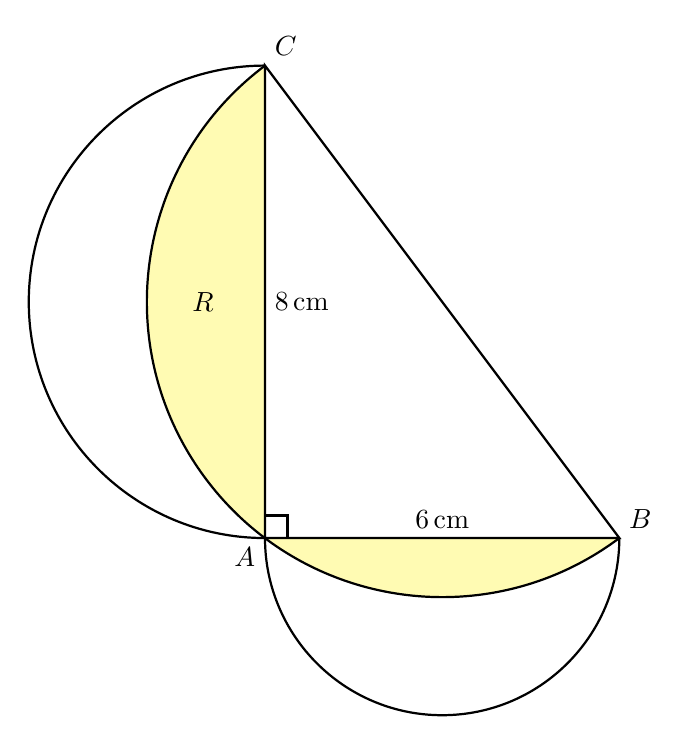
\begin{tikzpicture}[scale=0.75]
\def\AB{6}
\def\AC{8}
\def\ra{0.38}
\pgfmathsetmacro{\rAB}{\AB/2}
\pgfmathsetmacro{\rAC}{\AC/2}
\pgfmathsetmacro{\rBC}{sqrt(\AB*\AB+\AC*\AC)/2}
\pgfmathsetmacro{\alphaang}{atan(\AC/\AB)}
\pgfmathsetmacro{\angB}{-\alphaang}
\pgfmathsetmacro{\angA}{\alphaang-180}
\pgfmathsetmacro{\angC}{-\alphaang-180}

\coordinate (A) at (0,0);
\coordinate (B) at (\AB,0);
\coordinate (C) at (0,\AC);

% Region R: the part of the large semicircle outside triangle ABC
\path[fill=yellow!30]
  (A) -- (B)
  arc[start angle=\angB,end angle=\angA,radius=\rBC]
  -- cycle;

\path[fill=yellow!30]
  (A) -- (C)
  arc[start angle=\angC,end angle=\angA,radius=\rBC]
  -- cycle;

% Three semicircular arcs
\draw[thick, black] (A) arc[start angle=180,end angle=360,radius=\rAB];
\draw[thick, black] (A) arc[start angle=-90,end angle=-270,radius=\rAC];
\draw[thick, black] (B) arc[start angle=\angB,end angle=\angC,radius=\rBC];

% Triangle and diameters
\draw[thick, black] (A) -- (B) -- (C) -- cycle;

% Right-angle marker
\coordinate (RAx) at ($(A)+(\ra,0)$);
\coordinate (RAxy) at ($(A)+(\ra,\ra)$);
\coordinate (RAy) at ($(A)+(0,\ra)$);
\draw[thick] (RAx) -- (RAxy) -- (RAy);

% Labels
\node[below left] at (A) {$A$};
\node[above right] at (B) {$B$};
\node[above right] at (C) {$C$};
\path (A) -- node[midway, above] {$6\,\mathrm{cm}$} (B);
\path (A) -- node[midway, right] {$8\,\mathrm{cm}$} (C);
\node at (-1.05,4.0) {$R$};
\end{tikzpicture}
% end q000569 figure F1
\end{djsSolutionFigure}

The area of \(R\) is therefore
\[
R=\frac{25\pi}{2}-24
\]

The two smaller semicircles have radii \(3\) and \(4\), so their combined area is
\[
\frac12\pi(3^2)+\frac12\pi(4^2)
=\frac{25\pi}{2}
\]

The required shaded regions are precisely the parts of these two smaller semicircles that remain after removing \(R\). Hence their total area is
\[
\frac{25\pi}{2}-R
=\frac{25\pi}{2}-\left(\frac{25\pi}{2}-24\right)
=24
\]

Thus the total shaded area is \(24\,\mathrm{cm}^2\), exactly the same as the area of triangle \(ABC\).

The correct option is \textbf{B}. \\

\textit{Remark:} (optional)

This geometry is not special to the \(6\)-\(8\)-\(10\) triangle. 

For any right-angled triangle, the area of a semicircle is proportional to the square of its diameter, so Pythagoras gives:
\[
\text{area of the two semicircles on the shorter sides}
=
\text{area of the semicircle on the hypotenuse}
\]

Subtracting the parts common to these semicircles leaves the two curved regions outside the hypotenuse semicircle on one side, and the original right-angled triangle on the other. Hence the two curved regions always have total area equal to the area of the triangle.

These regions are known as the \emph{lunes of Hippocrates}. The result is a classical example of a curved shape whose area can be found exactly by reducing it to the area of a rectilinear figure. 

It is also closely connected to the Pythagorean theorem: the familiar relation
\[
a^2+b^2=c^2
\]
can equally well be expressed using the areas of any three similar figures constructed on the sides of a right-angled triangle, including semicircles.
% end q000569 solution
\end{djsSolution}
\end{enumerate}
\clearpage
\thispagestyle{djssolutions}
\vspace*{8pt}
\djsTopicLine{Coordinate Geometry}
\begin{enumerate}[label=\textbf{\arabic*.},leftmargin=*,itemsep=0pt,start=8]
\questionitem[Coordinate Geometry]
% begin q000629 stem
The line $y=3x+2$ meets the parabola $y=x^2$ at the points $P$ and $Q$. 

The tangents to the parabola at $P$ and $Q$ meet at $R$, as shown.

What are the coordinates of $R$?
% end q000629 stem

\begin{center}
% begin q000629 diagram
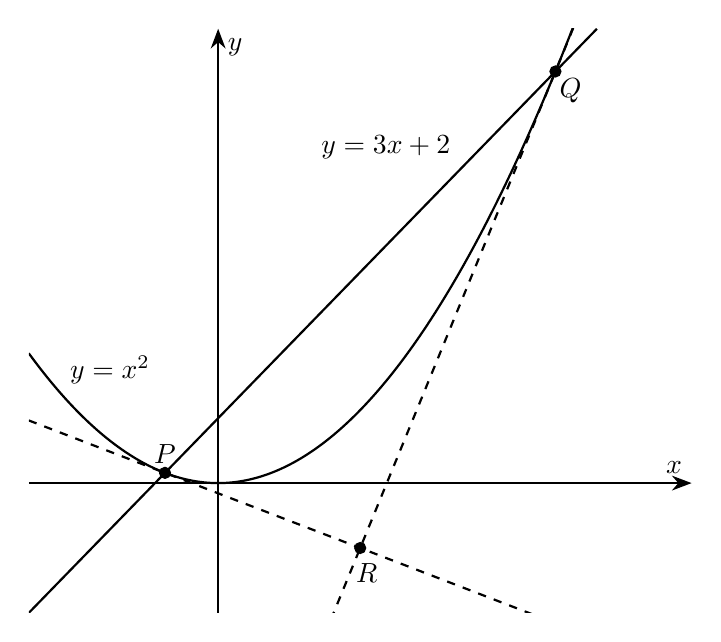
\begin{tikzpicture}
\pgfmathsetmacro{\px}{(3-sqrt(17))/2}
\pgfmathsetmacro{\qx}{(3+sqrt(17))/2}
\pgfmathsetmacro{\py}{(\px)*(\px)}
\pgfmathsetmacro{\qy}{(\qx)*(\qx)}
\pgfmathsetmacro{\rx}{(\px+\qx)/2}
\pgfmathsetmacro{\ry}{\px*\qx}

\pgfmathsetmacro{\curveLabelX}{-1.55}
\pgfmathsetmacro{\curveLabelY}{(\curveLabelX)*(\curveLabelX)}

\begin{axis}[
    width=10cm,
    height=9cm,
    axis lines=middle,
    axis line style={thick, black, -{Stealth[length=2.5mm]}},
    xlabel={$x$},
    ylabel={$y$},
    xmin=-2, xmax=5,
    ymin=-4, ymax=14,
    xtick=\empty,
    ytick=\empty,
    xticklabel=\empty,
    yticklabel=\empty,
    tick align=outside,
    enlargelimits=false,
    clip=true,
    samples=160
]

\coordinate (P) at (axis cs:\px,\py);
\coordinate (Q) at (axis cs:\qx,\qy);
\coordinate (R) at (axis cs:\rx,\ry);
\coordinate (curveLabel) at
    (axis cs:\curveLabelX,\curveLabelY);

% Parabola and secant
\addplot[thick, black, domain=-2:4, mark=none]
    {x^2};

\addplot[thick, black, domain=-2:4, samples=2, mark=none]
    {3*x+2}
    node[pos=0.76, above left] {$y=3x+2$};

% Tangents at P and Q
\addplot[dashed, black, thick, domain=-2:5, samples=2, mark=none]
    {2*(\px)*x-\py};

\addplot[dashed, black, thick, domain=-2:5, samples=2, mark=none]
    {2*(\qx)*x-\qy};

% Curve label
\node[above right, xshift=-4pt, yshift=4pt]
    at (curveLabel) {$y=x^2$};

% Marked points
\addplot[only marks, mark=*, mark size=2pt, black]
    coordinates {
        ({\px},{\py})
        ({\qx},{\qy})
        ({\rx},{\ry})
    };

\node[above, yshift=0pt] at (P) {$P$};
\node[below right, xshift=-2pt, yshift=1pt] at (Q) {$Q$};
\node[below right, xshift=-5pt, yshift=-2pt] at (R) {$R$};

\end{axis}
\end{tikzpicture}
% end q000629 diagram
\end{center}

\par\vspace*{12pt}
\begin{tabularx}{\linewidth}{@{}>{\bfseries}l Y@{}}
A &
% begin q000629 choice A
$\left(\dfrac{3}{2},-4\right)$
% end q000629 choice A
\\[0.8em]
B &
% begin q000629 choice B
$\left(\dfrac{3}{2},-2\right)$
% end q000629 choice B
\\[0.8em]
C &
% begin q000629 choice C
$\left(\dfrac{3}{2},-1\right)$
% end q000629 choice C
\\[0.8em]
D &
% begin q000629 choice D
$\left(3,-2\right)$
% end q000629 choice D
\\[0.8em]
E &
% begin q000629 choice E
$\left(1,-3\right)$
% end q000629 choice E
\\[0.8em]
F &
% begin q000629 choice F
$\left(2,-\dfrac{3}{2}\right)$
% end q000629 choice F
\\
\end{tabularx}

\begin{djsSolution}{B}
% begin q000629 solution
Let the $x$-coordinates of $P$ and $Q$ be $p$ and $q$ respectively.

Since $P$ and $Q$ lie on both $y=x^2$ and $y=3x+2$, their $x$-coordinates satisfy
\[
x^2=3x+2
\]
so
\[
x^2-3x-2=0
\]

Recall that the sum of the roots of a quadratic is
\(
-\tfrac{b}{a}
\)
and the product of the roots is
\(
\tfrac{c}{a}
\)

Hence, for $x^2-3x-2=0$,
\[
p+q=-\frac{-3}{1}=3
\]
and
\[
pq=\frac{-2}{1}=-2
\]

Since $\frac{\mathrm{d}y}{\mathrm{d}x}=2x$ the tangent to $y=x^2$ at the point $(p,p^2)$ has gradient $2p$, so its equation is
\[
y-p^2=2p(x-p)
\]
or
\[
y=2px-p^2
\]

Similarly, the tangent at $(q,q^2)$ is
\[
y=2qx-q^2
\]

At their intersection $R$, these two expressions for $y$ are equal, so
\[
2px-p^2=2qx-q^2
\]

Rearranging,
\[
2x(p-q)=p^2-q^2=(p-q)(p+q)
\]

Since $P$ and $Q$ are distinct, $p\ne q$, so
\[
x=\frac{p+q}{2}
\]

Thus the $x$-coordinate of $R$ is the average of the two roots. Since the sum of the roots is
\[
p+q=-\frac{b}{a}=3
\]
we have
\[
x=\frac32
\]

Substituting $x=\dfrac{p+q}{2}$ into the tangent at $P$ gives
\[
y=2p\left(\frac{p+q}{2}\right)-p^2
\]
so
\[
y=p(p+q)-p^2=pq
\]

Thus the $y$-coordinate of $R$ is the product of the two roots. Since
\[
pq=\frac{c}{a}=-2
\]
we have
\[
y=-2
\]

Hence
\[
R=\left(\frac32,-2\right)
\]

The correct option is \textbf{B}. \\[5pt]

\textit{Alternative Solution:} (brute force)

Instead of using the sum and product of the roots, we can find the points $P$ and $Q$ explicitly and then calculate the intersection of their tangents. We will see that this method proves to be quite painful. 

At $P$ and $Q$,
\[
x^2=3x+2
\]
so
\[
x^2-3x-2=0
\]

Using the quadratic formula,
\[
x=\frac{3\pm\sqrt{17}}{2}
\]

Hence
\[
P=\left(\frac{3-\sqrt{17}}{2},
\left(\frac{3-\sqrt{17}}{2}\right)^2\right)
\]
and
\[
Q=\left(\frac{3+\sqrt{17}}{2},
\left(\frac{3+\sqrt{17}}{2}\right)^2\right)
\]

Squaring the $x$-coordinates gives
\[
P=\left(\frac{3-\sqrt{17}}{2},
\frac{13-3\sqrt{17}}{2}\right)
\]
and
\[
Q=\left(\frac{3+\sqrt{17}}{2},
\frac{13+3\sqrt{17}}{2}\right)
\]

Since
\[
\frac{\mathrm{d}y}{\mathrm{d}x}=2x
\]
the gradient of the tangent at $P$ is
\[
3-\sqrt{17}
\]
and the gradient of the tangent at $Q$ is
\[
3+\sqrt{17}
\]

Using the tangent equation $y=2tx-t^2$ at a point $(t,t^2)$, the tangent at $P$ is
\[
y=(3-\sqrt{17})x-\frac{13-3\sqrt{17}}{2}
\]
while the tangent at $Q$ is
\[
y=(3+\sqrt{17})x-\frac{13+3\sqrt{17}}{2}
\]

At their intersection $R$, the two values of $y$ are equal, so
\[
(3-\sqrt{17})x-\frac{13-3\sqrt{17}}{2}
=
(3+\sqrt{17})x-\frac{13+3\sqrt{17}}{2}
\]

Rearranging gives
\[
3\sqrt{17}=2\sqrt{17}\,x
\]
and therefore
\[
x=\frac32
\]

Substituting into either tangent equation,
\[
y=(3-\sqrt{17})\frac32-\frac{13-3\sqrt{17}}{2}
\]
so
\[
y=\frac{9-3\sqrt{17}-13+3\sqrt{17}}{2}=-2
\]

Hence
\[
R=\left(\frac32,-2\right)
\]

So we again obtain option \textbf{B} but with considerably more pain and suffering. \\[5pt]

\textit{Remark:} (optional)

There is a general property of parabolas behind the calculation above. 

If two points on a parabola have $x$-coordinates $p$ and $q$, then the tangents at those points meet at a point whose $x$-coordinate is
\[
\frac{p+q}{2}
\]

This is the same as the $x$-coordinate of the midpoint of the chord joining the two points. 

Geometrically, the intersection of the two tangents and the midpoint of the chord therefore lie on a line parallel to the axis of the parabola.
% end q000629 solution
\end{djsSolution}
\end{enumerate}
\clearpage
\thispagestyle{djssolutions}
\vspace*{8pt}
\djsTopicLine{Logic}
\begin{enumerate}[label=\textbf{\arabic*.},leftmargin=*,itemsep=0pt,start=9]
\questionitem[Logic]
% begin q000161 stem
Consider the statement ($\ast$):

\[ \begin{array}{c}
\text{\textbf{If} $0 \le f(x) \le 1$ for all real $x$ with $0 \le x \le 1$, \textbf{then}}\\[5pt]

\text{$\displaystyle\int_0^1 f(x)\,\mathrm{d}x \le \int_0^1 (f(x))^2\,\mathrm{d}x$} \\[10pt]
\end{array} \tag{$\ast$} \] Which of the following functions is a \textbf{counterexample} to ($\ast$)?
% end q000161 stem

\par\vspace*{12pt}
\begin{tabularx}{\linewidth}{@{}>{\bfseries}l Y@{}}
A &
% begin q000161 choice A
$f(x)=2x$
% end q000161 choice A
\\[0.8em]
B &
% begin q000161 choice B
$f(x)=x^2+\frac{1}{2}$
% end q000161 choice B
\\[0.8em]
C &
% begin q000161 choice C
$f(x)=1$
% end q000161 choice C
\\[0.8em]
D &
% begin q000161 choice D
$f(x)=1+x$
% end q000161 choice D
\\[0.8em]
E &
% begin q000161 choice E
$f(x)=0$
% end q000161 choice E
\\[0.8em]
F &
% begin q000161 choice F
$f(x)=5x(1-x)$
% end q000161 choice F
\\[0.8em]
G &
% begin q000161 choice G
$f(x)=\sqrt{x}+\frac{1}{2}$
% end q000161 choice G
\\[0.8em]
H &
% begin q000161 choice H
$f(x)=\frac12$
% end q000161 choice H
\\
\end{tabularx}

\begin{djsSolution}{H}
% begin q000161 solution
A counterexample to a statement of the form ``if A, then B'' must make the antecedent A true and the consequent B false.

Here, the antecedent is the condition
\[
0\leq f(x)\leq1
\]
for every \(x\) with \(0\leq x\leq1\)

The consequent is the inequality
\[
\int_0^1 f(x)\,\mathrm{d}x
\leq
\int_0^1 (f(x))^2\,\mathrm{d}x
\]

So a function that fails the inequality \(0\leq f(x)\leq1\) cannot be a counterexample, regardless of what happens to its integrals. It is therefore quickest to check the antecedent first.

At \(x=1\), four options immediately fail:
\[
\begin{aligned}
\text{A:}\quad f(1)&=2(1)=2>1\\
\text{B:}\quad f(1)&=1^2+\frac12=\frac32>1\\
\text{D:}\quad f(1)&=1+1=2>1\\
\text{G:}\quad f(1)&=\sqrt{1}+\frac12=\frac32>1
\end{aligned}
\]

Option F also fails the antecedent inequality. Taking \(x=\frac12\),
\[
f\left(\frac12\right)
=
5\left(\frac12\right)\left(1-\frac12\right)
=
\frac54>1
\]

Thus A, B, D, F and G all make the antecedent false, so none of them can be a counterexample.

This leaves C, E and H. These are the constant functions
\[
f(x)=1,\qquad f(x)=0,\qquad f(x)=\frac12
\]
and all three satisfy \(0\leq f(x)\leq1\) throughout \(0\leq x\leq1\)

For C,
\[
f(x)=1
\quad\Longrightarrow\quad
(f(x))^2=1
\]
so
\[
\int_0^1 f(x)\,\mathrm{d}x
=
\int_0^1 (f(x))^2\,\mathrm{d}x
=
1
\]

The required inequality is true, so C is not a counterexample.

Similarly, for E,
\[
f(x)=0
\quad\Longrightarrow\quad
(f(x))^2=0
\]
and therefore
\[
\int_0^1 f(x)\,\mathrm{d}x
=
\int_0^1 (f(x))^2\,\mathrm{d}x
=
0
\]

Again, the required inequality is true, so E is not a counterexample.

For H, \(f(x)=\frac12\), so the antecedent is certainly true. However,
\[
\int_0^1\frac12\,\mathrm{d}x
=
\frac12
\]
whereas
\[
\int_0^1\left(\frac12\right)^2\,\mathrm{d}x
=
\int_0^1\frac14\,\mathrm{d}x
=
\frac14
\]

The claimed conclusion would therefore require
\[
\frac12\leq\frac14
\]
which is false.

Thus \textbf{H} makes the antecedent true and the consequent false, so it is a counterexample to the statement.
% end q000161 solution
\end{djsSolution}
\end{enumerate}
\clearpage
\thispagestyle{djssolutions}
\vspace*{8pt}
\djsTopicLine{Logic}
\begin{enumerate}[label=\textbf{\arabic*.},leftmargin=*,itemsep=0pt,start=10]
\questionitem[Logic]
% begin q000687 stem
Consider the following three conditions on a positive real number $x$

\[
\begin{array}{@{}ll@{}}
(1) & x^2 - 3x + 2 < 0 \\[5pt]
(2) & \log_{10} x > 0 \\[5pt]
(3) & 2^x > 4 \\[5pt]
\end{array}\]

Which of the following statements is/are true?

\[
\begin{array}{@{}l l@{}}
\textbf{I:} & \text{Condition (2) holds only if at least one of conditions (1) and (3) holds} \\[8pt]
\textbf{II:} & \text{If condition (2) does not hold, then condition (3) does not hold} \\[8pt]
\textbf{III:} &
\begin{aligned}[t]
&\text{For condition (1) to hold, it is necessary but not sufficient} \\
&\text{that condition (3) does not hold} \\[5pt]
\end{aligned}
\end{array}
\]
% end q000687 stem

\par\vspace*{12pt}
\begin{tabularx}{\linewidth}{@{}>{\bfseries}l Y@{}}
A &
% begin q000687 choice A
None of them
% end q000687 choice A
\\[0.8em]
B &
% begin q000687 choice B
I only
% end q000687 choice B
\\[0.8em]
C &
% begin q000687 choice C
II only
% end q000687 choice C
\\[0.8em]
D &
% begin q000687 choice D
III only
% end q000687 choice D
\\[0.8em]
E &
% begin q000687 choice E
I and II only
% end q000687 choice E
\\[0.8em]
F &
% begin q000687 choice F
I and III only
% end q000687 choice F
\\[0.8em]
G &
% begin q000687 choice G
II and III only
% end q000687 choice G
\\[0.8em]
H &
% begin q000687 choice H
I, II and III
% end q000687 choice H
\\
\end{tabularx}

\begin{djsSolution}{G}
% begin q000687 solution
First translate each of the three conditions into a simple condition on \(x\).

For condition (1),
\[
x^2-3x+2<0
\]
so
\[
(x-1)(x-2)<0
\]

The product is negative between the two roots, hence
\[
(1)\qquad 1<x<2
\]

For condition (2), since \(\log_{10}x\) is increasing and \(\log_{10}1=0\),
\[
\log_{10}x>0
\]
is equivalent to
\[
(2)\qquad x>1
\]

For condition (3), since \(4=2^2\) and \(2^x\) is increasing,
\[
2^x>4
\]
is equivalent to
\[
(3)\qquad x>2
\]

So the three conditions are simply
\[
\begin{array}{@{}ll@{}}
(1)&1<x<2\\[3pt]
(2)&x>1\\[3pt]
(3)&x>2
\end{array}
\]

We can now translate each statement into ordinary inequalities.

For statement I, the phrase ``condition (2) holds only if at least one of conditions (1) and (3) holds'' means
\[
\text{if (2) holds, then (1) or (3) must hold}
\]

In terms of \(x\), this says
\[
x>1
\quad\Longrightarrow\quad
1<x<2\ \text{or}\ x>2
\]

This is almost true, but \(x=2\) is missed. At \(x=2\), condition (2) holds because \(2>1\), but condition (1) does not hold because \(2\not<2\), and condition (3) does not hold because \(2\not>2\).

Therefore statement I is false.

For statement II,
\[
\text{if condition (2) does not hold, then condition (3) does not hold}
\]

Since \(x\) is positive, condition (2) not holding means
\[
0<x\leq1
\]

Condition (3) not holding means
\[
x\leq2
\]

So statement II is asking whether
\[
0<x\leq1
\quad\Longrightarrow\quad
x\leq2
\]

This is always true. Therefore statement II is true.

For statement III, first recall what ``necessary'' and ``sufficient'' mean.

Saying that \(A\) is \textbf{necessary} for \(B\) means that \(B\) cannot hold without \(A\), or equivalently
\[
B\Longrightarrow A
\]

Saying that \(A\) is \textbf{sufficient} for \(B\) means that \(A\) guarantees \(B\), or equivalently
\[
A\Longrightarrow B
\]

Here, statement III says that for condition (1) to hold, it is necessary but not sufficient that condition (3) does not hold.

Condition (1) is
\[
1<x<2
\]

Condition (3) does not hold when
\[
x\leq2
\]

For \(x\leq2\) to be \textbf{necessary} for \(1<x<2\), we need
\[
1<x<2
\quad\Longrightarrow\quad
x\leq2
\]

This is true.

For \(x\leq2\) to be \textbf{not sufficient}, it must fail to guarantee \(1<x<2\). For example, \(x=1\) satisfies
\[
x\leq2
\]
but does not satisfy
\[
1<x<2
\]

So condition (3) not holding is necessary for condition (1), but it is not sufficient.

Therefore statement III is true.

Statements II and III are true, while statement I is false, so the correct option is \textbf{G}.
% end q000687 solution
\end{djsSolution}
\end{enumerate}
\clearpage
\thispagestyle{djssolutions}
\vspace*{8pt}
\djsTopicLine{Probability \& Counting}
\begin{enumerate}[label=\textbf{\arabic*.},leftmargin=*,itemsep=0pt,start=11]
\questionitem[Probability \& Counting]
% begin q000596 stem
A three-digit code is formed by selecting three different digits from $1,2,3,4,5,6$ and placing them in random order. 

Each possible code is equally likely.

It is revealed that when the three digits in the code are multiplied together, the result is divisible by $6$.

What is the probability that the code contains the digit $6$?
% end q000596 stem

\par\vspace*{12pt}
\begin{tabularx}{\linewidth}{@{}>{\bfseries}l Y@{}}
A &
% begin q000596 choice A
$\dfrac{1}{3}$
% end q000596 choice A
\\[0.8em]
B &
% begin q000596 choice B
$\dfrac{1}{2}$
% end q000596 choice B
\\[0.8em]
C &
% begin q000596 choice C
$\dfrac{3}{5}$
% end q000596 choice C
\\[0.8em]
D &
% begin q000596 choice D
$\dfrac{2}{3}$
% end q000596 choice D
\\[0.8em]
E &
% begin q000596 choice E
$\dfrac{3}{4}$
% end q000596 choice E
\\[0.8em]
F &
% begin q000596 choice F
$\dfrac{5}{6}$
% end q000596 choice F
\\
\end{tabularx}

\begin{djsSolution}{D}
% begin q000596 solution
We are told that the product of the three chosen digits is divisible by \(6\). Since
\[
6=2\times3
\]
the selected digits must supply both a factor of \(2\) and a factor of \(3\).

It is convenient to count \emph{sets of three digits} rather than ordered codes. Each set of three distinct digits can be arranged in exactly
\[
3!=6
\]
different orders, so every valid selection gives the same number of codes. The ordering therefore does not affect the required probability.

First count the valid selections that contain \(6\).

Once \(6\) is chosen, the product is automatically divisible by \(6\), because the digit \(6\) itself supplies both a factor of \(2\) and a factor of \(3\). We only need to choose the other two digits from \(1,2,3,4,5\), giving
\[
\binom{5}{2}=10
\]
valid selections containing \(6\).

Now count the valid selections that do not contain \(6\).

The available digits are then
\[
1,2,3,4,5
\]
and the product must still contain a factor of \(3\). The only available multiple of \(3\) is \(3\), so \(3\) must be selected.

We therefore choose the other two digits from
\[
1,2,4,5
\]

There are
\[
\binom{4}{2}=6
\]
ways to do this altogether. However, the pair \(\{1,5\}\) contains no even digit, so the selection \(\{1,3,5\}\) has no factor of \(2\) and its product is not divisible by \(6\).

Thus the number of valid selections not containing \(6\) is
\[
6-1=5
\]

So, among the selections whose product is divisible by \(6\), there are
\[
10+5=15
\]
possible selections in total, of which \(10\) contain the digit \(6\).

Hence the required conditional probability is
\[
\frac{10}{15}=\frac23
\]

The correct option is \textbf{D}.
% end q000596 solution
\end{djsSolution}
\end{enumerate}
\clearpage
\thispagestyle{djssolutions}
\vspace*{8pt}
\djsTopicLine{Proof \& Error Analysis}
\begin{enumerate}[label=\textbf{\arabic*.},leftmargin=*,itemsep=0pt,start=12]
\questionitem[Proof \& Error Analysis]
% begin q000678 stem
Consider the claim about cubic polynomials: \\[-5pt]

\noindent\hbox to \linewidth{%
  \hfil
  \llap{\textbf{Claim:}\hspace{0.4em}}%
  \parbox[t]{0.7\linewidth}{\centering
    If a cubic polynomial $f$ has distinct roots $a$, $b$ and $c$, where $a<b<c$, then there exists $x$ with $a<x<b$ such that $f''(x)=0$}%
  \hfil} \\

The student attempts to prove the claim and produces the following argument:
\[
\begin{array}{@{}rl@{}}
\mathbf{I} & \text{Since } f(a)=f(b)=0,\text{ there is a number }p\text{ such that }a<p<b\text{ and }f'(p)=0 \\[5pt]
\mathbf{II} & \text{Similarly, there is a number }q\text{ such that }b<q<c\text{ and }f'(q)=0 \\[5pt]
\mathbf{III} & \text{The polynomial }f'\text{ is quadratic with roots }p\text{ and }q,\text{ so }f''\!\left(\frac{p+q}{2}\right)=0 \\[5pt]
\mathbf{IV} &
\text{Since }a<p<b<q<c,\text{ we have }p-b<0<q-b,\text{ and hence}\\[4pt]
&\displaystyle\qquad
\frac{p+q}{2}-b
=\frac{(p-b)+(q-b)}{2}<0 \\[5pt]
\mathbf{V} & \text{Therefore the claim is true, the claimed } x \text{ can be chosen as } x=\frac{p+q}{2}\\[5pt]
\end{array}
\]

Which line contains the first error?
% end q000678 stem

\par\vspace*{12pt}
\begin{tabularx}{\linewidth}{@{}>{\bfseries}l Y@{}}
A &
% begin q000678 choice A
Line $\mathbf{I}$
% end q000678 choice A
\\[0.8em]
B &
% begin q000678 choice B
Line $\mathbf{II}$
% end q000678 choice B
\\[0.8em]
C &
% begin q000678 choice C
Line $\mathbf{III}$
% end q000678 choice C
\\[0.8em]
D &
% begin q000678 choice D
Line $\mathbf{IV}$
% end q000678 choice D
\\[0.8em]
E &
% begin q000678 choice E
Line $\mathbf{V}$
% end q000678 choice E
\\[0.8em]
F &
% begin q000678 choice F
There is no error, the proof is correct as written.
% end q000678 choice F
\\
\end{tabularx}

\begin{djsSolution}{D}
% begin q000678 solution
Lines I and II are valid:

Between the consecutive roots \(a\) and \(b\), the graph of the cubic lies entirely on one side of the \(x\)-axis. Since it starts on the axis at \(x=a\) and returns to the axis at \(x=b\), it must turn somewhere between them. Hence there is some \(p\) with
\[
a<p<b
\]
such that
\[
f'(p)=0
\]

The same reasoning between the consecutive roots \(b\) and \(c\) gives some \(q\) with
\[
b<q<c
\]
such that
\[
f'(q)=0
\]

So Lines I and II are correct.

Line III is also correct. Since \(f\) is cubic, \(f'\) is quadratic, and we have just found its two roots \(p\) and \(q\).

The turning point of a quadratic lies halfway between its roots, so the turning point of \(f'\) has \(x\)-coordinate
\[
\frac{p+q}{2}
\]

At a turning point of \(f'\), its gradient is zero. Since the gradient of \(f'\) is \(f''\),
\[
f''\!\left(\frac{p+q}{2}\right)=0
\]

The first error occurs in Line IV:

From
\[
p<b<q
\]
we certainly have
\[
p-b<0
\qquad\text{and}\qquad
q-b>0
\]

But one of these numbers is negative and the other is positive, so we cannot determine the sign of their sum.

For example, it could be that
\[
p-b=-1
\qquad\text{and}\qquad
q-b=2
\]
in which case
\[
(p-b)+(q-b)=1>0
\]

It could instead be negative, or it could be zero. Therefore
\[
\frac{(p-b)+(q-b)}{2}<0
\]
does not follow from the information given.

So Line IV has not shown that
\[
\frac{p+q}{2}<b
\]

The point where \(f''(x)=0\) is halfway between \(p\) and \(q\), but that midpoint could lie on either side of \(b\), or even be equal to \(b\).

Therefore the first error is in Line IV, so the correct option is \textbf{D}.\\[5pt]

\textit{Remark:} (optional)

The claim itself is actually false. For example, take
\[
f(x)=x^3-x
\]

Its three distinct roots are
\[
-1,\quad 0,\quad 1
\]
so here
\[
a=-1,\qquad b=0,\qquad c=1
\]

Differentiating twice gives
\[
f'(x)=3x^2-1
\]
and
\[
f''(x)=6x
\]

Hence
\[
f''(x)=0
\]
only when
\[
x=0
\]

But \(x=0\) is exactly \(b\), not a value between \(a\) and \(b\). Thus there is no \(x\) with
\[
-1<x<0
\]
for which \(f''(x)=0\)

So the student's argument fails at Line IV, and in this case it is attempting to prove a claim which is itself false.
% end q000678 solution
\end{djsSolution}
\end{enumerate}
\clearpage
\thispagestyle{djssolutions}
\vspace*{8pt}
\djsTopicLine{Integration}
\begin{enumerate}[label=\textbf{\arabic*.},leftmargin=*,itemsep=0pt,start=13]
\questionitem[Integration]
% begin q000120 stem
For each positive integer $n$, define \[ F(n)=\int_0^1 x^n\,\mathrm{d}x \] and \[ H(n)=\sum_{r=1}^n \frac{1}{F(r)} \]

What is the smallest positive integer $n$ such that $H(n)>15$?
% end q000120 stem

\par\vspace*{12pt}
\begin{tabularx}{\linewidth}{@{}>{\bfseries}l Y@{}}
A &
% begin q000120 choice A
$3$
% end q000120 choice A
\\[0.8em]
B &
% begin q000120 choice B
$4$
% end q000120 choice B
\\[0.8em]
C &
% begin q000120 choice C
$5$
% end q000120 choice C
\\[0.8em]
D &
% begin q000120 choice D
$6$
% end q000120 choice D
\\[0.8em]
E &
% begin q000120 choice E
$7$
% end q000120 choice E
\\
\end{tabularx}

\begin{djsSolution}{C}
% begin q000120 solution
First evaluate \(F(r)\):
\[
F(r)=\int_0^1 x^r\,\mathrm{d}x
=\left[\frac{x^{r+1}}{r+1}\right]_0^1
=\frac{1}{r+1}
\]

Therefore
\[
\frac{1}{F(r)}=r+1
\]
and hence
\[
H(n)=2+3+4+\cdots+(n+1)
\]

This is an arithmetic series with first term \(a=2\), common difference \(d=1\), and \(n\) terms.

For an arithmetic series, one form of the sum formula is
\[
S_n=\frac{n}{2}\bigl[2a+(n-1)d\bigr]
\]

Another equivalent form, if the last term is \(l\), is
\[
S_n=\frac{n}{2}(a+l)
\]

Using the first formula with \(a=2\) and \(d=1\),
\[
H(n)
=\frac{n}{2}\bigl[2(2)+(n-1)(1)\bigr]
\]

Therefore
\[
H(n)
=\frac{n}{2}(n+3)
=\frac{n(n+3)}{2}
\]

We require
\[
H(n)>15
\]
so
\[
\frac{n(n+3)}{2}>15
\]

Multiplying by \(2\),
\[
n(n+3)>30
\]
and therefore
\[
n^2+3n-30>0
\]

The corresponding quadratic equation has roots
\[
n=\frac{-3\pm\sqrt{3^2-4(1)(-30)}}{2}
=\frac{-3\pm\sqrt{129}}{2}
\]

Only the positive root is relevant. Since
\[
11^2<129<12^2
\]
we have
\[
11<\sqrt{129}<12
\]
and hence
\[
4<\frac{-3+\sqrt{129}}{2}<\frac92
\]

The quadratic is positive for values of \(n\) greater than this positive root, so the smallest positive integer that works is
\[
n=5
\]

The correct option is \textbf{C}.\\[5pt]

\textit{Alternative Solution:}

After finding
\[
F(r)=\frac{1}{r+1}
\]
we have
\[
H(n)=\sum_{r=1}^{n}(r+1)
\]

Split this into two standard sums:
\[
H(n)=\sum_{r=1}^{n}r+\sum_{r=1}^{n}1
\]

Recall that
\[
\sum_{r=1}^{n}r=\frac{n(n+1)}{2}
\]
and, since the sum contains \(n\) copies of \(1\),
\[
\sum_{r=1}^{n}1=n
\]

Therefore
\[
H(n)
=\frac{n(n+1)}{2}+n
=\frac{n(n+3)}{2}
\]

We need
\[
\frac{n(n+3)}{2}>15
\]
or equivalently
\[
n(n+3)>30
\]

Since the answers are consecutive integers, it is quicker here to test the relevant options than to solve the quadratic.

For \(n=4\),
\[
n(n+3)=4(7)=28<30
\]
so \(n=4\) is too small.

For \(n=5\),
\[
n(n+3)=5(8)=40>30
\]
so \(n=5\) works.

Also, each additional term in \(H(n)\) is positive, so \(H(n)\) increases as \(n\) increases. Since \(n=4\) fails and \(n=5\) works, the smallest possible value is \(n=5\).

The correct option is \textbf{C}.
% end q000120 solution
\end{djsSolution}
\end{enumerate}
\clearpage
\thispagestyle{djssolutions}
\vspace*{8pt}
\djsTopicLine{Logic}
\begin{enumerate}[label=\textbf{\arabic*.},leftmargin=*,itemsep=0pt,start=14]
\questionitem[Logic]
% begin q000125 stem
Let $S$ be the statement: \[ \begin{array}{c}
\text{For all real numbers $x$, if $|x| \ge 1$ then $g(x) > 0$}
\end{array} \] Which of the following is a correct \textbf{negation} of $S$?
% end q000125 stem

\par\vspace*{12pt}
\begin{tabularx}{\linewidth}{@{}>{\bfseries}l Y@{}}
A &
% begin q000125 choice A
There exists a real number $x$ with $|x| \ge 1$ such that $g(x) \le 0$
% end q000125 choice A
\\[0.8em]
B &
% begin q000125 choice B
There exists a real number $x$ with $|x| > 1$ such that $g(x) < 0$
% end q000125 choice B
\\[0.8em]
C &
% begin q000125 choice C
For all real numbers $x$, either $|x| < 1$ or $g(x) > 0$
% end q000125 choice C
\\[0.8em]
D &
% begin q000125 choice D
For all real numbers $x$ with $|x| \ge 1$, $g(x) \ge 0$
% end q000125 choice D
\\[0.8em]
E &
% begin q000125 choice E
There exists a real number $x$ such that $|x| < 1$ and $g(x) \le 0$
% end q000125 choice E
\\[0.8em]
F &
% begin q000125 choice F
There exists a real number $x$ such that $|x| < 1$ or $g(x) \le 0$
% end q000125 choice F
\\
\end{tabularx}

\begin{djsSolution}{A}
% begin q000125 solution
There are two standard rules for negating statements of this kind.

First, negating a statement about \textbf{all} values changes
\[
\text{``for all''}\quad\longleftrightarrow\quad\text{``there exists''}
\]
So the negation of
\[
\text{For all real numbers }x,\ \ldots
\]
must begin
\[
\text{There exists a real number }x\text{ such that }\ldots
\]

We now need to negate what follows.

For a statement of the form
\[
\text{if A, then B}
\]
the negation is
\[
\text{A and not B}
\]

This is closely connected to the idea of a counterexample. To show that ``if A, then B'' is false, we need an example for which A really does hold, but B fails.

Here,
\[
\text{A: }\quad|x|\geq1
\]
and
\[
\text{B:}\quad g(x)>0
\]

Therefore the negation of the implication is
\[
|x|\geq1
\quad\text{and}\quad
\text{not}\bigl(g(x)>0\bigr)
\]

The negation of \(g(x)>0\) is
\[
g(x)\leq0
\]

The equality case is important: if \(g(x)=0\), then \(g(x)>0\) is already false.

Putting the two negation rules together, the negation of the original statement is
\[
\text{There exists a real number }x\text{ such that }|x|\geq1
\text{ and }g(x)\leq0
\]

In other words, the negation says that there is at least one counterexample to the original claim.

The correct option is \textbf{A}.
% end q000125 solution
\end{djsSolution}
\end{enumerate}
\clearpage
\thispagestyle{djssolutions}
\vspace*{8pt}
\djsTopicLine{Proof \& Error Analysis}
\begin{enumerate}[label=\textbf{\arabic*.},leftmargin=*,itemsep=0pt,start=15]
\questionitem[Proof \& Error Analysis]
% begin q000682 stem
A function $f$ is defined for all real $x$, and $f'(x)$ exists for every real $x$.

The function $f$ is also \textbf{strictly increasing:} whenever $a<b$, also $f(a)<f(b)$.

A student makes the following claim:
\begin{center}
\begin{minipage}{0.82\linewidth}
\centering
\textbf{Claim:} It follows that $f'(x)>0$ for every real $x$
\end{minipage}
\end{center}
The student argues as follows:

\[
\begin{array}{@{}rl@{}}
\textbf{Line 1:} & \text{Suppose, for a contradiction, that $f'(c)\le 0$ for some real number $c$} \\[5pt]
\textbf{Line 2:} & \text{If $f'(c)<0$, then just to the right of $c$ the graph of $f$ falls below} \\ 
& \text{$f(c)$, which contradicts $f$ being strictly increasing. Hence $f'(c)=0$} \\[5pt]
\textbf{Line 3:} & \text{So the tangent to the graph of $f$ at $x=c$ is horizontal} \\[5pt]
\textbf{Line 4:} & \text{A horizontal tangent at $x=c$ means there are numbers $a<c<b$ with} \\ 
& \text{$f(a)\ge f(c)$ or with $f(b)\le f(c)$} \\[5pt]
\textbf{Line 5:} & \text{Either possibility contradicts $f$ being strictly increasing. Hence} \\ 
& \text{$f'(x)>0$ for every real $x$} \\[5pt]
\end{array}
\]

Which of the following best describes the argument?
% end q000682 stem

\par\vspace*{12pt}
\begin{tabularx}{\linewidth}{@{}>{\bfseries}l Y@{}}
A &
% begin q000682 choice A
The argument is correct, and the claim is true
% end q000682 choice A
\\[0.8em]
B &
% begin q000682 choice B
The first error occurs in Line 2
% end q000682 choice B
\\[0.8em]
C &
% begin q000682 choice C
The first error occurs in Line 3
% end q000682 choice C
\\[0.8em]
D &
% begin q000682 choice D
The first error occurs in Line 4
% end q000682 choice D
\\[0.8em]
E &
% begin q000682 choice E
The first error occurs in Line 5
% end q000682 choice E
\\[0.8em]
F &
% begin q000682 choice F
The argument contains an error, but the claim is nevertheless true
% end q000682 choice F
\\
\end{tabularx}

\begin{djsSolution}{D}
% begin q000682 solution
Line 1 is a valid way to begin a proof by contradiction. The student assumes that
\[
f'(c)\leq0
\]
for some real number \(c\)

Line 2 is also correct. If
\[
f'(c)<0
\]
then the graph is sloping downwards at \(x=c\). Moving a sufficiently small distance to the right of \(c\) would therefore make the value of \(f\) smaller than \(f(c)\). This is impossible for a strictly increasing function.

Hence, under the assumption in Line 1, the only remaining possibility is
\[
f'(c)=0
\]

Line 3 is therefore correct. If
\[
f'(c)=0
\]
then the tangent to the graph at \(x=c\) has gradient \(0\), so it is horizontal.

The first error is in Line 4.

A horizontal tangent does not imply either of the inequalities claimed there. Consider
\[
f(x)=x^3
\]
and take
\[
c=0
\]

Then
\[
f'(x)=3x^2
\]
so
\[
f'(0)=0
\]

Thus the tangent at \(x=0\) is horizontal.

However, for any \(a<0<b\),
\[
f(a)=a^3<0=f(0)<b^3=f(b)
\]

Therefore
\[
f(a)<f(c)
\]
and
\[
f(b)>f(c)
\]

So neither
\[
f(a)\geq f(c)
\]
nor
\[
f(b)\leq f(c)
\]
holds.

This directly contradicts the assertion made in Line 4, so Line 4 is the first error.

The same example also shows that the original claim is false: \(f(x)=x^3\) is strictly increasing, but
\[
f'(0)=0
\]

Therefore the first error occurs in Line 4, so the correct option is \textbf{D}.
% end q000682 solution
\end{djsSolution}
\end{enumerate}
\clearpage
\thispagestyle{djssolutions}
\vspace*{8pt}
\djsTopicLine{Sequences \& Series}
\begin{enumerate}[label=\textbf{\arabic*.},leftmargin=*,itemsep=0pt,start=16]
\questionitem[Sequences \& Series]
% begin q000531 stem
Let $n$ be an integer with $n \ge 6$. 

In the expansion of $(1+x)^n$ the coefficients of $x^4$, $x^5$ and $x^6$, in that order, are consecutive terms of an arithmetic sequence.

What is the sum of all possible values of $n$?
% end q000531 stem

\par\vspace*{12pt}
\begin{tabularx}{\linewidth}{@{}>{\bfseries}l Y@{}}
A &
% begin q000531 choice A
$13$
% end q000531 choice A
\\[0.8em]
B &
% begin q000531 choice B
$14$
% end q000531 choice B
\\[0.8em]
C &
% begin q000531 choice C
$20$
% end q000531 choice C
\\[0.8em]
D &
% begin q000531 choice D
$21$
% end q000531 choice D
\\[0.8em]
E &
% begin q000531 choice E
$22$
% end q000531 choice E
\\[0.8em]
F &
% begin q000531 choice F
$28$
% end q000531 choice F
\\
\end{tabularx}

\begin{djsSolution}{D}
% begin q000531 solution
By the binomial theorem,
\[
(1+x)^n
=
\binom{n}{0}
+\binom{n}{1}x
+\binom{n}{2}x^2
+\cdots
+\binom{n}{r}x^r
+\cdots
\]

Therefore the coefficients of \(x^4\), \(x^5\) and \(x^6\) are respectively
\[
\binom{n}{4},
\qquad
\binom{n}{5},
\qquad
\binom{n}{6}
\]

Note that the notation \(\binom{n}{r}\) is also sometimes written \({}^nC_r\).

Since these three coefficients are consecutive terms of an arithmetic sequence, their successive differences must be equal:
\[
\binom{n}{5}-\binom{n}{4}
=
\binom{n}{6}-\binom{n}{5}
\]

Rearranging,
\[
2\binom{n}{5}
=
\binom{n}{4}+\binom{n}{6}
\]

Using
\[
\binom{n}{r}
=
\frac{n!}{r!(n-r)!}
\]
gives
\[
2\left(\frac{n!}{5!(n-5)!}\right)
=
\frac{n!}{4!(n-4)!}
+
\frac{n!}{6!(n-6)!}
\]

Since \(n!\neq0\), we can divide every term by \(n!\):
\[
\frac{2}{5!(n-5)!}
=
\frac{1}{4!(n-4)!}
+
\frac{1}{6!(n-6)!}
\]

Now multiply throughout by \((n-4)!\):
\[
\frac{2(n-4)!}{5!(n-5)!}
=
\frac{(n-4)!}{4!(n-4)!}
+
\frac{(n-4)!}{6!(n-6)!}
\]

The middle term simplifies immediately:
\[
\frac{(n-4)!}{4!(n-4)!}
=
\frac{1}{4!}
\]

For the first term,
\[
(n-4)!=(n-4)(n-5)!
\]
so
\[
\frac{(n-4)!}{(n-5)!}
=
n-4
\]

For the final term,
\[
(n-4)!=(n-4)(n-5)(n-6)!
\]
so
\[
\frac{(n-4)!}{(n-6)!}
=
(n-4)(n-5)
\]

Hence
\[
\frac{2(n-4)}{5!}
=
\frac{1}{4!}
+
\frac{(n-4)(n-5)}{6!}
\]

Multiplying throughout by \(6!\) gives
\[
\frac{2\cdot6!}{5!}(n-4)
=
\frac{6!}{4!}
+
(n-4)(n-5)
\]

Now
\[
\frac{6!}{5!}=6
\]
and
\[
\frac{6!}{4!}=6\cdot5=30
\]
so
\[
12(n-4)
=
30+(n-4)(n-5)
\]

Expanding,
\[
12n-48
=
30+n^2-9n+20
\]

Therefore
\[
n^2-21n+98=0
\]

Factorising,
\[
(n-7)(n-14)=0
\]

Thus
\[
n=7
\qquad\text{or}\qquad
n=14
\]

Both values satisfy \(n\geq6\), so the sum of all possible values of \(n\) is
\[
7+14=21
\]

The correct option is \textbf{D}.

\medskip

Once the quadratic
\[
n^2-21n+98=0
\]
has been obtained, the question can also be finished without factorising. For a quadratic \(ax^2+bx+c=0\), the sum of the roots is
\[
-\frac{b}{a}
\]
so here the sum of the two possible values of \(n\) is immediately
\[
-\frac{-21}{1}=21
\]
% end q000531 solution
\end{djsSolution}
\end{enumerate}
\clearpage
\thispagestyle{djssolutions}
\vspace*{8pt}
\djsTopicLine{Logic}
\begin{enumerate}[label=\textbf{\arabic*.},leftmargin=*,itemsep=0pt,start=17]
\questionitem[Logic]
% begin q000686 stem
Let $a$ be a real number. Consider the following statement:

\begin{center}
\begin{minipage}{0.8\textwidth}
\centering
For all real numbers $x$, there exists a real number $y$ such that\\

$a\le y\le a+\pi$ and $\sin y=\sin x$
\end{minipage}
\end{center}

Which condition on $a$ is \textbf{necessary and sufficient} for the statement to be true?
% end q000686 stem

\par\vspace*{12pt}
\begin{tabularx}{\linewidth}{@{}>{\bfseries}l Y@{}}
A &
% begin q000686 choice A
$\sin a=0$
% end q000686 choice A
\\[0.8em]
B &
% begin q000686 choice B
$\cos a=0$
% end q000686 choice B
\\[0.8em]
C &
% begin q000686 choice C
$\sin 2a=0$
% end q000686 choice C
\\[0.8em]
D &
% begin q000686 choice D
$\cos 2a=0$
% end q000686 choice D
\\[0.8em]
E &
% begin q000686 choice E
$\sin a=\cos a$
% end q000686 choice E
\\[0.8em]
F &
% begin q000686 choice F
$\sin a=-\cos a$
% end q000686 choice F
\\
\end{tabularx}

\begin{djsSolution}{B}
% begin q000686 solution
As \(x\) runs through all real numbers, \(\sin x\) takes every value from \(-1\) to \(1\).

So the statement is asking for the interval
\[
a\leq y\leq a+\pi
\]
to contain enough of the sine graph for \(\sin y\) to take every possible value between \(-1\) and \(1\).

In particular, the interval must contain some point where
\[
\sin y=1
\]
and also some point where
\[
\sin y=-1
\]

These are respectively a maximum and a minimum of the sine graph.

\begin{djsSolutionFigure}
% begin q000686 figure F1
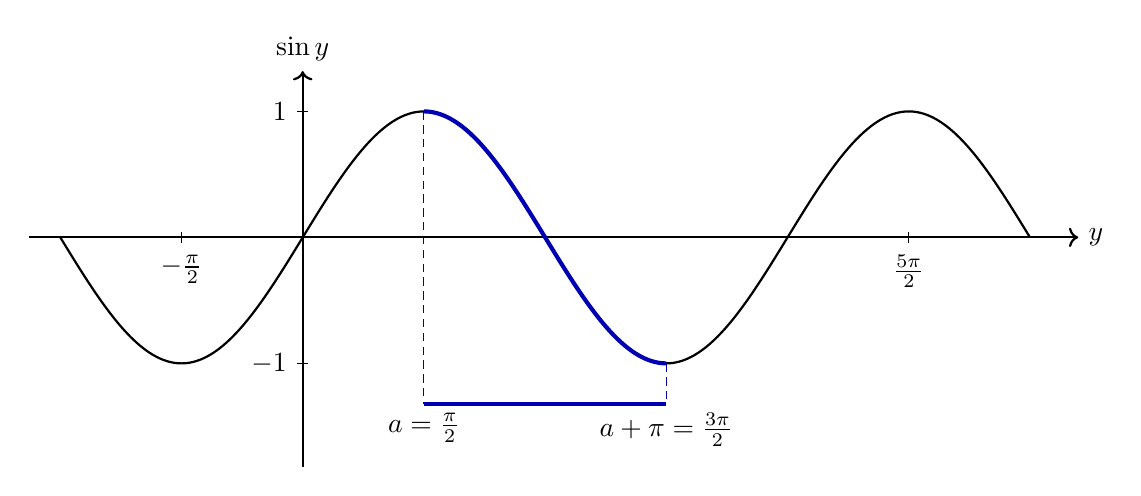
\begin{tikzpicture}[x=0.98cm,y=1.6cm]
\pgfmathsetmacro{\pival}{pi}
\pgfmathsetmacro{\leftneighbor}{-\pival/2}
\pgfmathsetmacro{\leftend}{\pival/2}
\pgfmathsetmacro{\rightend}{3*\pival/2}
\pgfmathsetmacro{\rightneighbor}{5*\pival/2}
\pgfmathsetmacro{\graphend}{3*\pival}
\def\intervalheight{-1.32}

\draw[blue!70!black, densely dashed] (\leftend,1) -- (\leftend,\intervalheight);
\draw[blue!70!black, densely dashed] (\rightend,-1) -- (\rightend,\intervalheight);
\draw[->,thick] (-3.55,0) -- (10.05,0) node[right] {$y$};
\draw[->,thick] (0,-1.82) -- (0,1.32) node[above] {$\sin y$};
\draw[thick,black,domain=-\pival:\graphend,samples=200,smooth,variable=\t]
    plot (\t,{sin(deg(\t))});
\draw[blue!70!black,line width=1.5pt,domain=\leftend:\rightend,samples=100,smooth,variable=\t]
    plot (\t,{sin(deg(\t))});
\draw[blue!70!black,line width=1.5pt] (\leftend,\intervalheight) -- (\rightend,\intervalheight);

\draw (\leftneighbor,-0.045) -- (\leftneighbor,0.045);
\draw (\rightneighbor,-0.045) -- (\rightneighbor,0.045);
\draw (-0.07,1) -- (0.07,1);
\draw (-0.07,-1) -- (0.07,-1);
\node[below] at (\leftneighbor,-0.06) {$-\frac{\pi}{2}$};
\node[below] at (\rightneighbor,-0.06) {$\frac{5\pi}{2}$};
\node[left] at (-0.08,1) {$1$};
\node[left] at (-0.08,-1) {$-1$};
\node[below] at (\leftend,\intervalheight) {$a=\frac{\pi}{2}$};
\node[below] at (\rightend,\intervalheight) {$a+\pi=\frac{3\pi}{2}$};
\end{tikzpicture}
% end q000686 figure F1
\end{djsSolutionFigure}

Successive maxima and minima of the sine graph are \(\pi\) apart. For example,
\[
\sin\left(\frac{\pi}{2}\right)=1
\]
and
\[
\sin\left(\frac{3\pi}{2}\right)=-1
\]

More generally, a maximum and the neighbouring minimum are always separated by exactly \(\pi\).

But the interval from \(a\) to \(a+\pi\) also has length exactly \(\pi\). Therefore, if it is to contain both a maximum and a minimum, these two points must occur at the two endpoints of the interval.

Hence
\[
\sin a=1
\]
and
\[
\sin(a+\pi)=-1
\]
or else
\[
\sin a=-1
\]
and
\[
\sin(a+\pi)=1
\]

In either case,
\[
\sin a=\pm1
\]

Using
\[
\sin^2a+\cos^2a=1
\]
we obtain
\[
\cos^2a=1-\sin^2a=0
\]
so
\[
\cos a=0
\]

Thus \(\cos a=0\) is a necessary condition.

We must also check that it is sufficient.

Suppose
\[
\cos a=0
\]

Then
\[
\sin a=\pm1
\]

So \(a\) is a maximum or a minimum of the sine graph. Since increasing the input by \(\pi\) changes the sign of the sine,
\[
\sin(a+\pi)=-\sin a
\]

Therefore \(a+\pi\) is the neighbouring minimum or maximum.

As \(y\) moves from \(a\) to \(a+\pi\), the sine graph moves continuously from \(1\) to \(-1\), or from \(-1\) to \(1\). Hence it takes every value between \(-1\) and \(1\).

Since \(\sin x\) must always lie between \(-1\) and \(1\), for every real \(x\) there is therefore some \(y\) with
\[
a\leq y\leq a+\pi
\]
such that
\[
\sin y=\sin x
\]

So \(\cos a=0\) is both necessary and sufficient.

The correct option is \textbf{B}.
% end q000686 solution
\end{djsSolution}
\end{enumerate}
\clearpage
\thispagestyle{djssolutions}
\vspace*{8pt}
\djsTopicLine{Logic}
\begin{enumerate}[label=\textbf{\arabic*.},leftmargin=*,itemsep=0pt,start=18]
\questionitem[Logic]
% begin q000683 stem
Let $p$ and $q$ be real constants, and let
\[f(x)=x^3+px^2+qx\] Consider the statement 
\begin{center}
\begin{minipage}{0.82\linewidth}
\centering
S: \, There exists a real number $x$ such that $f'(x)<0$
\end{minipage}
\end{center}
Which of the following conditions is \textbf{necessary} but \textbf{not sufficient} for S?
% end q000683 stem

\par\vspace*{12pt}
\begin{tabularx}{\linewidth}{@{}>{\bfseries}l Y@{}}
A &
% begin q000683 choice A
$q<0$
% end q000683 choice A
\\[0.8em]
B &
% begin q000683 choice B
$q\le 0$
% end q000683 choice B
\\[0.8em]
C &
% begin q000683 choice C
$3q<p^2$
% end q000683 choice C
\\[0.8em]
D &
% begin q000683 choice D
$3q\le p^2$
% end q000683 choice D
\\[0.8em]
E &
% begin q000683 choice E
$p^2>0$
% end q000683 choice E
\\[0.8em]
F &
% begin q000683 choice F
$p^2\ge 3|q|$
% end q000683 choice F
\\
\end{tabularx}

\begin{djsSolution}{D}
% begin q000683 solution
First translate the logic in the question.

A condition is \textbf{necessary} for S if S cannot be true without that condition also being true.

A condition is \textbf{not sufficient} for S if the condition can be true while S is false.

So we are looking for a condition which must hold whenever there is some real \(x\) with
\[
f'(x)<0
\]
but which does not, by itself, guarantee that such an \(x\) exists.

Differentiate:
\[
f'(x)=3x^2+2px+q
\]

Since \(f'(x)\) is a quadratic with positive \(x^2\)-coefficient, it has a minimum. Completing the square makes that minimum easy to identify:
\[
\begin{aligned}
f'(x)
&=3x^2+2px+q\\
&=3\left(x^2+\frac{2p}{3}x\right)+q\\
&=3\left(x+\frac{p}{3}\right)^2-\frac{p^2}{3}+q
\end{aligned}
\]

Thus
\[
f'(x)
=
3\left(x+\frac{p}{3}\right)^2
+
q-\frac{p^2}{3}
\]

The squared term is always non-negative, and it is \(0\) when
\[
x=-\frac{p}{3}
\]

Therefore the minimum possible value of \(f'(x)\) is
\[
q-\frac{p^2}{3}
\]

For there to exist some real \(x\) for which \(f'(x)<0\), this minimum must be strictly negative:
\[
q-\frac{p^2}{3}<0
\]

Multiplying by \(3\) gives
\[
3q<p^2
\]

So S is true exactly when
\[
3q<p^2
\]

This means option C is both necessary \emph{and} sufficient for S, so it is not the answer being asked for.

Now consider option D:
\[
3q\leq p^2
\]

Whenever S is true, we have
\[
3q<p^2
\]
which certainly implies
\[
3q\leq p^2
\]

So option D is necessary.

However, it is not sufficient, because equality is also allowed. For example, take
\[
p=0,\qquad q=0
\]

Then
\[
3q\leq p^2
\]
is true, since both sides are \(0\). But
\[
f'(x)=3x^2
\]
and therefore
\[
f'(x)\geq0
\]
for every real \(x\)

So there is no real \(x\) for which \(f'(x)<0\), and S is false.

Thus \(3q\leq p^2\) is necessary but not sufficient for S.

The correct option is \textbf{D}.
% end q000683 solution
\end{djsSolution}
\end{enumerate}
\clearpage
\thispagestyle{djssolutions}
\vspace*{8pt}
\djsTopicLine{Algebra}
\begin{enumerate}[label=\textbf{\arabic*.},leftmargin=*,itemsep=0pt,start=19]
\questionitem[Algebra]
% begin q000589 stem
A real number $x$ satisfies
\[
x^2-3x+1=0
\]
What is the value of $x^6+\dfrac{1}{x^6}$?
% end q000589 stem

\par\vspace*{12pt}
\begin{tabularx}{\linewidth}{@{}>{\bfseries}l Y@{}}
A &
% begin q000589 choice A
$288$
% end q000589 choice A
\\[0.8em]
B &
% begin q000589 choice B
$306$
% end q000589 choice B
\\[0.8em]
C &
% begin q000589 choice C
$320$
% end q000589 choice C
\\[0.8em]
D &
% begin q000589 choice D
$322$
% end q000589 choice D
\\[0.8em]
E &
% begin q000589 choice E
$324$
% end q000589 choice E
\\
\end{tabularx}

\begin{djsSolution}{D}
% begin q000589 solution
The expression
\[
x^6+\frac{1}{x^6}
\]
contains matching positive and negative powers of \(x\). This suggests trying to find
\[
x+\frac{1}{x}
\]
rather than solving explicitly for \(x\).

We are given
\[
x^2-3x+1=0
\]

Since \(x=0\) does not satisfy this equation, we may divide throughout by \(x\):
\[
x-3+\frac{1}{x}=0
\]

Hence
\[
x+\frac{1}{x}=3
\]

Now square both sides:
\[
\left(x+\frac{1}{x}\right)^2=3^2
\]

Expanding,
\[
x^2+2+\frac{1}{x^2}=9
\]

Therefore
\[
x^2+\frac{1}{x^2}=7
\]

Square again:
\[
\left(x^2+\frac{1}{x^2}\right)^2=7^2
\]

Expanding,
\[
x^4+2+\frac{1}{x^4}=49
\]

Hence
\[
x^4+\frac{1}{x^4}=47
\]

We now have expressions involving the second and fourth powers. Multiplying them produces the sixth powers:
\[
\left(x^2+\frac{1}{x^2}\right)
\left(x^4+\frac{1}{x^4}\right)
\]

Expanding,
\[
x^6+x^2+\frac{1}{x^2}+\frac{1}{x^6}
\]

Using
\[
x^2+\frac{1}{x^2}=7
\]
this becomes
\[
x^6+\frac{1}{x^6}+7
\]

But the product is also
\[
7\times47=329
\]

Therefore
\[
x^6+\frac{1}{x^6}+7=329
\]

so
\[
x^6+\frac{1}{x^6}=322
\]

The correct option is \textbf{D}.\\[5pt]

\textit{Remark:} (exam technique)

Questions of this form are often traps in disguise. It is possible to solve the quadratic first and then substitute
\[
x=\frac{3\pm\sqrt5}{2}
\]
but raising either of these expressions to the sixth power would create a large amount of unnecessary algebra.

The paired form
\[
x^n+\frac{1}{x^n}
\]
is the important clue. When the original equation has a non-zero constant term, dividing by a suitable power of \(x\) can often reveal an expression such as
\[
x+\frac{1}{x}
\]
which can then be used to build the required higher powers.

In a timed test, questions like this can consume a disproportionate amount of time if the intended simplification is not spotted. Before committing to a long calculation, it is worth checking whether the form of the required expression suggests a shorter route.
% end q000589 solution
\end{djsSolution}
\end{enumerate}
\clearpage
\thispagestyle{djssolutions}
\vspace*{8pt}
\djsTopicLine{Polynomials}
\begin{enumerate}[label=\textbf{\arabic*.},leftmargin=*,itemsep=0pt,start=20]
\questionitem[Polynomials]
% begin q000619 stem
The equation \[x^3 - 3x + p = 0\] where $p$ is a real constant, has three distinct real solutions for $x$.

Find the complete set of values of $p$
% end q000619 stem

\par\vspace*{12pt}
\begin{tabularx}{\linewidth}{@{}>{\bfseries}l Y@{}}
A &
% begin q000619 choice A
$-3 < p < 3$
% end q000619 choice A
\\[0.8em]
B &
% begin q000619 choice B
$-2 < p < 2$
% end q000619 choice B
\\[0.8em]
C &
% begin q000619 choice C
$-2 \le p \le 2$
% end q000619 choice C
\\[0.8em]
D &
% begin q000619 choice D
$p < -2$ or $p > 2$
% end q000619 choice D
\\[0.8em]
E &
% begin q000619 choice E
$0 < p < 4$
% end q000619 choice E
\\[0.8em]
F &
% begin q000619 choice F
$-4 < p < 0$
% end q000619 choice F
\\
\end{tabularx}

\begin{djsSolution}{B}
% begin q000619 solution
Let
\[
f(x)=x^3-3x+p
\]

The real solutions of
\[
x^3-3x+p=0
\]
are exactly the \(x\)-coordinates where the graph of \(y=f(x)\) crosses or touches the \(x\)-axis.

To have three distinct real solutions, the cubic must therefore meet the \(x\)-axis at three different points.

First find the stationary points:
\[
f'(x)=3x^2-3
\]

Setting \(f'(x)=0\),
\[
3x^2-3=0
\]
so
\[
x^2=1
\]
and hence
\[
x=-1
\qquad\text{or}\qquad
x=1
\]

The cubic rises to a local maximum at \(x=-1\), then falls to a local minimum at \(x=1\).

Their heights are
\[
f(-1)=(-1)^3-3(-1)+p=p+2
\]
and
\[
f(1)=1^3-3(1)+p=p-2
\]

So the stationary points are
\[
(-1,p+2)
\qquad\text{and}\qquad
(1,p-2)
\]

\begin{djsSolutionFigure}
% begin q000619 figure F1
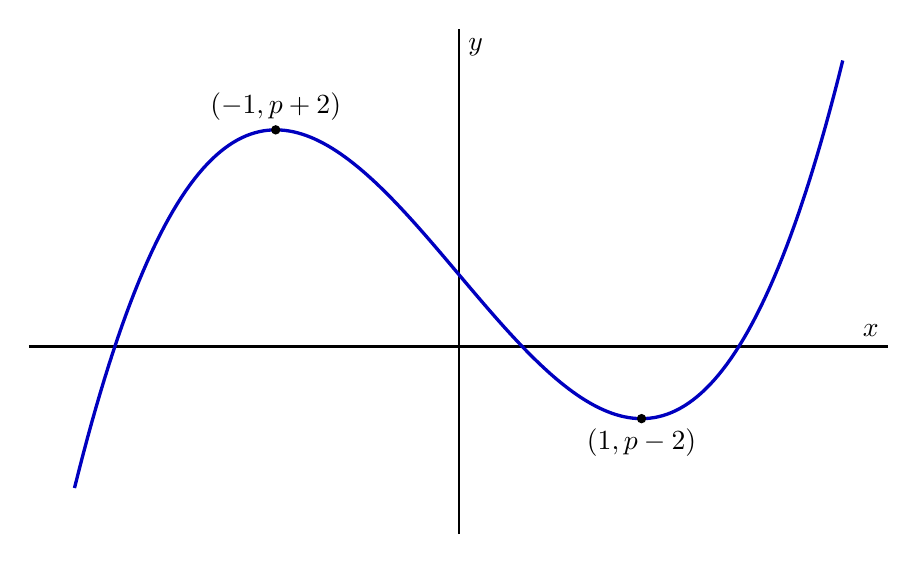
\begin{tikzpicture}
\begin{axis}[
    width=12.5cm, height=8cm,
    xmin=-2.35, xmax=2.35,
    ymin=-2.6, ymax=4.4,
    axis lines=middle,
    axis line style={black, thick, -},
    xlabel={$x$}, ylabel={$y$},
    xtick=\empty, ytick=\empty,
    clip=true
]
\addplot[very thick, blue!75!black, domain=-2.1:2.1, samples=180]
    {x^3-3*x+1};
\fill[black] (axis cs:-1,3) circle (1.7pt);
\fill[black] (axis cs:1,-1) circle (1.7pt);
\node[above] at (axis cs:-1,3) {$(-1,p+2)$};
\node[below] at (axis cs:1,-1) {$(1,p-2)$};
\end{axis}
\end{tikzpicture}
% end q000619 figure F1
\end{djsSolutionFigure}

Since the coefficient of \(x^3\) is positive, the graph eventually goes downwards without bound to the left and upwards without bound to the right.

For the graph to cross the \(x\)-axis three times, its local maximum must lie above the \(x\)-axis, while its local minimum must lie below the \(x\)-axis.

Therefore we require
\[
p+2>0
\]
and
\[
p-2<0
\]

The first inequality gives
\[
p>-2
\]

The second gives
\[
p<2
\]

Combining these,
\[
-2<p<2
\]

The inequalities must be strict. For example, if \(p=2\), then the local minimum lies exactly on the \(x\)-axis:
\[
f(1)=0
\]
so the graph touches the axis at \(x=1\) rather than crossing it there. This produces a repeated root, not three distinct real roots.

Similarly, \(p=-2\) makes the local maximum lie on the \(x\)-axis and again gives a repeated root.

Hence the complete set of values is
\[
-2<p<2
\]

The correct option is \textbf{B}.
% end q000619 solution
\end{djsSolution}
\end{enumerate}
\end{document}
